\documentclass[11pt,a4paper]{report}

% Packages
\usepackage[utf8]{inputenc}
\usepackage[T1]{fontenc}
\usepackage[english]{babel}
\usepackage[default]{sourcesanspro} % Modern sans-serif font
\usepackage{graphicx}
\usepackage{amssymb}
\usepackage{amsmath}
\usepackage{hyperref}
\usepackage{geometry}
\usepackage{titlesec}
\usepackage{fancyhdr}
\usepackage{booktabs}
\usepackage{multirow}
\usepackage{float}
\usepackage{listings}
\usepackage{xcolor}
\usepackage{tikz}
\usepackage[most,skins]{tcolorbox}
\usepackage{titletoc}
\usepackage{setspace} % For line spacing
\usepackage{caption}  % For caption styling
\usepackage{subcaption} % For subfigures
\usepackage{enumitem} % For list customization
\usepackage{amssymb} % For math symbols like \mathbb
\usetikzlibrary{calc, fadings, shadows.blur, shapes.geometric}

% Typography & Spacing
\setstretch{1.15} % Slightly increased line spacing
\setlength{\parskip}{1em} % Increased spacing between paragraphs
\setlength{\parindent}{0pt} % No indentation

% Caption Styling
\captionsetup{
    font={small, color=textGray},
    labelfont={bf, color=primaryPink},
    labelsep=endash,
    margin=10pt
}

% List Styling - Compact
\setlist[itemize]{label=\textcolor{primaryPink}{\textbullet}, leftmargin=*, itemsep=0pt, topsep=2pt, parsep=0pt}
\setlist[enumerate]{label=\textcolor{primaryPink}{\textbf{\arabic*.}}, leftmargin=*, itemsep=0pt, topsep=2pt, parsep=0pt}

% Custom Info Boxes - Minimalist
\newtcolorbox{infobox}[1][]{
    colback=white,
    colframe=textGray,
    coltitle=textDark,
    title={\textbf{Insight}},
    fonttitle=\bfseries\small,
    arc=0mm,
    boxrule=0.5pt,
    left=5pt, right=5pt, top=2pt, bottom=2pt,
    #1
}

\newtcolorbox{note}[1][]{
    colback=white,
    colframe=textGray,
    coltitle=textDark,
    title={\textbf{Note}},
    fonttitle=\bfseries\small,
    arc=0mm,
    boxrule=0.5pt,
    left=5pt, right=5pt, top=2pt, bottom=2pt,
    #1
}


% Geometry - Balanced
\geometry{
    left=2.0cm,
    right=2.0cm,
    top=2.0cm,
    bottom=2.0cm
}
\setlength{\headheight}{25pt}

% Colors (Extracted from HTML)
\definecolor{primaryPink}{RGB}{194, 24, 91}
\definecolor{accentPink}{RGB}{233, 30, 99}
\definecolor{textDark}{RGB}{26, 26, 26}
\definecolor{textGray}{RGB}{107, 114, 128}
\definecolor{bgLight}{RGB}{250, 250, 250}
\definecolor{cardBg}{RGB}{255, 255, 255}

% Hyperlinks
\hypersetup{
    colorlinks=true,
    linkcolor=primaryPink,
    filecolor=primaryPink,
    urlcolor=primaryPink,
    citecolor=primaryPink,
    pdftitle={OncoCare Project Report},
}

% Code listing style
\lstset{
    basicstyle=\ttfamily\small,
    breaklines=true,
    frame=single,
    keywordstyle=\color{primaryPink}\bfseries,
    commentstyle=\color{textGray},
    stringstyle=\color{green!50!black},
    backgroundcolor=\color{gray!10}
}

% Title Format - Compact
\titleformat{\chapter}[display]
  {\normalfont\huge\bfseries\color{textDark}}{\chaptertitlename\ \thechapter}{10pt}{\Huge}[\vspace{0.5ex}\color{primaryPink}\titlerule]
\titlespacing*{\chapter}{0pt}{-40pt}{10pt}

\titleformat{\section}
  {\normalfont\Large\bfseries\color{textDark}}{\color{primaryPink}\thesection}{1em}{}
\titlespacing*{\section}{0pt}{5pt}{2pt}

\titleformat{\subsection}
  {\normalfont\large\bfseries\color{textDark}}{\color{primaryPink}\thesubsection}{1em}{}
\titlespacing*{\subsection}{0pt}{5pt}{2pt}

% Table of Contents Styling
\titlecontents{chapter}[0em]
  {\addvspace{0.5pc}\bfseries\color{textDark}}
  {\color{textDark}\contentslabel[\thecontentslabel]{2em}}
  {}
  {\hfill\color{textDark}\bfseries\thecontentspage}

\titlecontents{section}[2em]
  {\addvspace{0.1pc}\color{textGray}}
  {\contentslabel{2.3em}}
  {}
  {\titlerule*[0.75pc]{.}\contentspage}

% Header and Footer
\pagestyle{fancy}
\fancyhf{}
\renewcommand{\headrulewidth}{0.5pt} % Thin header line
\renewcommand{\headrule}{\hbox to\headwidth{\color{textGray!50}\leaders\hrule height \headrulewidth\hfill}}
\fancyhead[L]{\textcolor{textGray}{\small\bfseries OncoCare}}
\fancyhead[R]{\textcolor{textGray}{\small \leftmark}}
\fancyfoot[C]{\textcolor{textGray}{\thepage}}

% Custom TColorBox for Cards
\newtcolorbox{metacard}[2][]{
    colback=cardBg,
    colframe=gray!20,
    width=#2,
    boxrule=1pt,
    arc=4mm,
    auto outer arc,
    boxsep=5pt,
    left=5pt, right=5pt, top=5pt, bottom=5pt,
    enhanced,
    fontupper=\centering,
    #1
}

\begin{document}

% --- COVER PAGE ---
\begin{titlepage}
    \newgeometry{left=0cm, right=0cm, top=0cm, bottom=0cm}
    \thispagestyle{empty}

    % --- Professional Background & Visuals ---
    \begin{tikzpicture}[remember picture, overlay]
        % 1. Premium Left Sidebar (Brand Color Gradient)
        \shade[top color=primaryPink, bottom color=accentPink] 
            (current page.north west) rectangle ([xshift=3cm]current page.south west);
        
        % 2. Sidebar Texture (Subtle Dots)
        \foreach \y in {-20,-19.5,...,20} {
             \fill[white, opacity=0.15] (1.5,\y) circle (0.8pt);
        }

        % 3. Top Right Geometric Accent
        \fill[primaryPink!5] 
            ([xshift=0cm, yshift=-12cm]current page.north east) 
            -- ([xshift=-12cm, yshift=0cm]current page.north east) 
            -- (current page.north east) -- cycle;

        % 4. Bottom Footer Bar (Dark Contrast)
        \fill[textDark] 
            ([xshift=3cm, yshift=0cm]current page.south west) rectangle (current page.south east);
            
        % 5. Abstract "Pink Ribbon" Flow (Subtle Background)
        \path[fill=primaryPink!2] 
            ([xshift=3cm, yshift=5cm]current page.south west) 
            .. controls ([xshift=8cm, yshift=15cm]current page.south west) and ([xshift=15cm, yshift=10cm]current page.south west) 
            .. (current page.north east) 
            -- ([xshift=3cm]current page.north east) -- cycle;
    \end{tikzpicture}

    % --- Content Layout ---
    \vspace{5cm} % Top Margin relative to page
    \hspace{5cm} % Left Margin (clear of sidebar)
    \begin{minipage}{0.75\textwidth}
        
        % Header: Institution & Context
        \begin{flushright}
            \vspace{-3cm}
            {\fontfamily{qhv}\selectfont\scriptsize\bfseries\color{textGray} ÉCOLE SUPÉRIEURE PRIVÉE D'INGÉNIERIE ET DE TECHNOLOGIE} \\
            {\fontfamily{qhv}\selectfont\tiny\bfseries\color{primaryPink} DÉPARTEMENT INFORMATIQUE — ANNÉE UNIVERSITAIRE 2025/2026}
            \vspace{3cm}
        \end{flushright}

        % Project Label
        {\fontfamily{qhv}\selectfont\scriptsize\bfseries\color{accentPink} \MakeUppercase{Projet de Recherche — Advanced Machine Learning}} \\
        \vspace{0.3cm}

        % Main Title (High Impact Typography)
        {\fontsize{40}{48}\selectfont\bfseries\color{textDark} Intelligent Breast \\ Cancer Diagnosis \\ \textcolor{primaryPink}{and Triage System} \par}
        
        \vspace{1.5cm}
        
        % Mission Statement / Subtitle (Styled Box)
        \begin{tcolorbox}[
            colback=white,
            colframe=primaryPink,
            leftrule=3pt,
            rightrule=0pt,
            toprule=0pt,
            bottomrule=0pt,
            arc=0mm,
            boxsep=0pt,
            left=15pt,
            width=\linewidth,
            nobeforeafter
        ]
            \color{textGray}\small\itshape
            "Un système d'aide à la décision clinique explicatif, conçu pour améliorer le triage précoce des lésions mammaires — en hommage à toutes les femmes touchées par le cancer du sein."
        \end{tcolorbox}

        \vspace{4.5cm}

        % Team & Supervisor Grid
        \begin{tabular}{@{}p{0.45\textwidth} p{0.45\textwidth}@{}}
            {\scriptsize\bfseries\color{textGray} ÉQUIPE DE PROJET} & {\scriptsize\bfseries\color{textGray} ENCADRANTE} \\
            \vspace{0.1cm} & \vspace{0.1cm} \\
            \textbf{Yasmine Chebbi} & \textbf{Mme Wiem Trabelsi} \\
            \textbf{Maram Chebbi} & \\
            \textbf{Malek Kammoun} & {\scriptsize\bfseries\color{textGray} CLASSE / MODULE} \\
            \textbf{Marwen Jnene} & 4DS11 — Advanced ML
        \end{tabular}

    \end{minipage}
    
    % --- Footer Info (On Dark Bar) ---
    \begin{tikzpicture}[remember picture, overlay]
        \node[text=white, font=\footnotesize\bfseries, anchor=east] at ([xshift=-1.5cm, yshift=1cm]current page.south east) {TUNIS, TUNISIE};
        \node[text=white, font=\footnotesize\bfseries, anchor=west] at ([xshift=4.5cm, yshift=1cm]current page.south west) {ESPRIT};
    \end{tikzpicture}
    
    \restoregeometry
\end{titlepage}



% Table of Contents
{
  \newgeometry{left=3cm,right=3cm,top=2.5cm,bottom=2.5cm} % Wider margins
  \hypersetup{linkcolor=textDark}
  \setlength{\parskip}{2pt} % Compact spacing
  \tableofcontents
  \newpage
  \listoffigures
  \listoftables
  \restoregeometry
}

% Chapters
\chapter{Introduction and Methodology}

\section{Project Context}
Breast cancer remains the most prevalent cancer among women worldwide, posing a significant global health challenge. Early and accurate diagnosis is the single most critical factor influencing patient survival rates. However, traditional diagnostic workflows—relying heavily on manual interpretation of mammography and histology—are resource-intensive, time-consuming, and subject to inter-observer variability.

\textbf{OncoCare} emerges as an intelligent Clinical Decision Support System (CDSS) designed to bridge the gap between medical expertise and computational precision. By automating risk stratification and providing predictive insights, OncoCare aims to assist oncologists in making faster, more evidence-based decisions. This project integrates advanced machine learning techniques to not only classify tumor malignancy with high sensitivity but also to predict tumor aggressiveness, thereby optimizing the triage process and prioritizing high-risk patients.

\section{Methodology}
This project adopts the \textbf{CRISP-DM} (Cross-Industry Standard Process for Data Mining) framework, ensuring a robust and medically aligned development lifecycle. The process is structured into five key phases:

\begin{table}[h]
    \centering
    \caption{CRISP-DM Project Methodology Phases}
    \renewcommand{\arraystretch}{1.5}
    \begin{tabular}{|p{0.3\textwidth}|p{0.65\textwidth}|}
        \hline
        \textbf{Phase} & \textbf{Content} \\
        \hline
        \textbf{Business Understanding} & We define the clinical objectives, focusing on minimizing False Negatives to ensure patient safety and optimizing triage workflows to reduce diagnostic delays. \\
        \hline
        \textbf{Data Understanding \& Preparation} & Leveraging the WBCD and METABRIC datasets, we perform rigorous exploratory analysis (EDA) and preprocessing. This includes handling class imbalance, feature scaling, and outlier detection. \\
        \hline
        \textbf{Modeling} & We develop and compare multiple architectures, ranging from interpretable linear models (Softmax Regression, SVM) to complex ensemble methods (XGBoost) and hybrid Neural Networks. \\
        \hline
        \textbf{Evaluation} & \textbf{WBCD (Diagnosis):} Validated using Accuracy, Sensitivity, Confusion Matrix, and ROC Curve. \newline \textbf{METABRIC (Prognosis):} Evaluated using R\textsuperscript{2}, RMSE, and MAE. \\
        \hline
        \textbf{Deployment} & The final solution is operationalized via a modern MLOps pipeline, featuring a FastAPI backend, static html frontend, and MLflow for experiment tracking. \\
        \hline
    \end{tabular}
\end{table}

\chapter{Business Understanding}


\section{Strategic Context \& Objectives}
\subsection{Problem Statement: The Diagnostic Gap}
Breast cancer remains the most prevalent cancer worldwide. Despite advancements, traditional diagnostic workflows are strained by rising patient volumes and human fatigue. Statistics from recent real-world studies underscore the urgency of AI integration:

\begin{itemize}
    \item \textbf{Efficiency Bottlenecks:} Pathological analysis often incurs a \textbf{7-14 day delay}, increasing patient anxiety and delaying critical treatment inception.
    \item \textbf{The Cost of Uncertainty:} Up to \textbf{20\% of cancers} can be missed in conventional screening, while \textbf{15-25\% of biopsies} performed are ultimately benign or unnecessary.
    \item \textbf{Proven Impact:} Deployed tools (e.g., Vara, MammoScreen) have demonstrated that AI-assisted workflows can increase detection rates by \textbf{17.6\%} while maintaining specificity, proving AI is a validated safety net.
\end{itemize}

\subsection{Stakeholder Analysis}
This system is designed not to replace, but to augment clinical expertise, targeting two primary stakeholders:

\begin{description}
    \item[Medical Professionals (Oncologists, Radiologists, Pathologists)] \hfill \\
    \textit{Objective: Clinical Decision Support (CDS).} To provide a reliable "second opinion" that reduces fatigue-related errors. The system automates routine morphological measurements, allowing the expert to focus on complex, edge-case diagnosis.
    
    \item[Healthcare Administration (Hospital Mgmt, Operations)] \hfill \\
    \textit{Objective: Resource Optimization.} To implement intelligent triage that dynamically routes high-probability cases to the front of the queue, maximizing the utilization of expensive diagnostic machinery (MRI/Biopsy) and specialist hours.
\end{description}

\section{BO 1: Classify Tumors for Rapid Diagnosis}

\begin{infobox}[title=Context]
In breast oncology, rapid and accurate differentiation between benign and malignant tumors is critical for patient outcomes. This AI system provides clinical decision support to optimize diagnostic accuracy and reduce unnecessary invasive procedures.
\end{infobox}

\subsection{Challenges}
\begin{itemize}
    \item \textbf{Medical Problem:} Diagnostic uncertainty leads to patient anxiety, delayed treatment for malignant cases, and unnecessary biopsies for benign masses.
    \item \textbf{Business Challenge:} Pathology bottlenecks delay diagnoses by 7-14 days. Senior pathologists waste time on routine cases.
    \item \textbf{AI Solution:} ML classifier predicting tumor malignancy from morphological features with $>97\%$ accuracy, enabling faster triage and ~20\% cost reduction.
\end{itemize}

\subsection{DSO 1: Binary Classification}
We developed three distinct architectures optimized for sensitivity and accuracy using morphological features from the WBCD dataset.

\begin{table}[H]
\centering
\small
\renewcommand{\arraystretch}{1.5}
\begin{tabular}{|p{0.25\textwidth}|p{0.35\textwidth}|p{0.3\textwidth}|}
\hline
\textbf{Model} & \textbf{Hyperparameters Configuration} & \textbf{Input Variables} \\
\hline
\textbf{Softmax Regression} \newline \textit{\textcolor{magenta}{Optimized}} & 
$\bullet$ $C = 10.0$ \newline
$\bullet$ solver = 'lbfgs' \newline
$\bullet$ max\_iter = 3000 \newline
$\bullet$ threshold = 0.477 
& \multirow{3}{=}{\textbf{30 Morphological Features:} \newline
$\bullet$ radius (mean/se/worst) \newline
$\bullet$ texture (mean/se/worst) \newline
$\bullet$ perimeter (mean/se/worst) \newline
$\bullet$ area (mean/se/worst) \newline
$\bullet$ smoothness (mean/se/worst) \newline
$\bullet$ compactness (mean/se/worst) \newline
$\bullet$ concavity (mean/se/worst) \newline
$\bullet$ concave points (mean/se/worst) \newline
$\bullet$ symmetry (mean/se/worst) \newline
$\bullet$ fractal dimension (mean/se/worst) \newline
\vspace{0.2cm}
\textbf{Target Variable:} \newline
diagnosis $\rightarrow$ Binary (B/M)} \\
\cline{1-2}
\textbf{GRU-SVM Hybrid} \newline \textit{\textcolor{magenta}{Optimized}} & 
\textbf{GRU Neural Network:} \newline
$\bullet$ units = 128 \newline
$\bullet$ dropout = 0.5 \newline
$\bullet$ learning\_rate = 0.001 \newline
\vspace{0.1cm}
\textbf{SVM Classifier:} \newline
$\bullet$ kernel = 'linear' \newline
$\bullet$ threshold = 0.25 
& \\
\cline{1-2}
\textbf{SVM-SGD} \newline \textit{\textcolor{magenta}{Optimized}} & 
$\bullet$ loss = 'hinge' (SVM loss) \newline
$\bullet$ penalty = 'l2' \newline
$\bullet$ alpha = $1/(5 \times n\_samples)$ \newline
$\bullet$ class\_weight = 'balanced' \newline
$\bullet$ learning\_rate = 'constant' \newline
$\bullet$ eta0 = 0.001 \newline
$\bullet$ max\_iter = 3000 \newline
$\bullet$ tol = 1e-4 \newline
$\bullet$ random\_state = 42 
& \\
\hline
\end{tabular}
\caption{Model Configurations for Binary Classification}
\label{tab:model_configurations}
\end{table}

\subsection{Success Metrics: Clinical Interpretation}
\begin{itemize}
    \item \textbf{Sensitivity (Recall):} \textit{Primary Safety Metric.} Measures the ability to identify all malignant cases. Maximizing this minimizes \textbf{False Negatives} (missed cancers), acting as the critical safety net for the diagnostic workflow.
    \item \textbf{False Negative Rate (FNR):} \textit{Risk Metric.} The inverse of sensitivity. Our "Challenger" model is selected specifically to drive this metric towards zero, ensuring no patient is incorrectly discharged.
    \item \textbf{Precision:} \textit{Efficiency Metric.} Balances the safety net by measuring how many predicted cancers are truly malignant. High precision minimizes \textbf{False Positives}, reducing unnecessary biopsies and patient anxiety.
    \item \textbf{Accuracy:} \textit{Global Metric.} Provides a baseline for overall reliability across the population but is secondary to sensitivity in this imbalanced clinical context.
\end{itemize}

\section{BO 2: Optimize Triage and Resource Allocation}

\begin{infobox}[title=Context]
We are designing an AI-powered triage system to prioritize cancer patients based on malignancy risk probability. This system replaces traditional "first-come-first-served" logistics with a data-driven prioritization engine.
\end{infobox}

\subsection{DSO 2.1: Probability Scoring and Calibration}
To ensure the reliability of risk estimates, the model's raw outputs are refined using \textbf{Sigmoid Calibration}. This process transforms the model's scores into true probabilities, ensuring that a predicted risk of 70\% corresponds to a true 70\% likelihood of malignancy.

\subsection{DSO 2.2: Explainability}
To build clinical trust, the system implements a dual-layer interpretability framework:

\subsubsection{Global Explainability}
We utilize \textbf{Model Coefficients} to provide a high-level overview of which features (e.g., Radius, Texture) generally drive predictions across the entire patient population.

\subsubsection{Local Explainability}
For individual patient cases, we employ \textbf{SHAP (SHapley Additive exPlanations)}. This technique breaks down a specific prediction, quantifying exactly how much each feature contributed to the final risk score, offering personalized transparency.

\subsection{DSO 2.3: Risk Stratification Logic}
The system employs a hybrid decision-making model integrating statistical predictions with clinical safety nets:

\begin{itemize}
    \item \textbf{Statistical Stratification:} Patients are categorized into five risk levels (Very Low to Critical) based on calibrated probabilities, guiding specific interventions.
    \item \textbf{Clinical Safety Net:} "Danger Flags" are triggered when physiological features breach safety thresholds.
    \item \textbf{Dynamic Escalation:} Patients with $\ge 2$ danger flags are automatically upgraded to the next risk tier.
    \item \textbf{Enhanced Prioritization:} A "Priority Queue" flags high-acuity cases ($\ge 80\%$ probability or multiple flags) to ensure immediate attention.
\end{itemize}

\section{BO 3: Personalize Treatment Strategies}

\begin{infobox}[title=Context]
Moving beyond binary diagnosis to characterize specific biological behavior (aggressiveness, growth velocity) for precision medicine. This section details the technical specifications for the METABRIC dataset model integration.
\end{infobox}

\subsection{DSO 3.1: Multi-Output Architecture \& Generalization}
Implementation of a \textbf{Gradient Boosting Multi-Output Regressor} designed to simultaneously predict three distinct clinical targets.

\begin{table}[H]
\centering
\small
\renewcommand{\arraystretch}{1.5}
\begin{tabular}{|p{0.2\textwidth}|p{0.35\textwidth}|p{0.35\textwidth}|}
\hline
\textbf{Component} & \textbf{Random Forest} & \textbf{Gradient Boosting} \\
\hline
\textbf{Architecture} & Multi-Output Regressor (RandomForestRegressor) & Multi-Output Regressor (GradientBoostingRegressor) \\
\hline
\textbf{Hyperparameters} & 
$\bullet$ n\_estimators = 200 \newline
$\bullet$ max\_depth = 10 \newline
$\bullet$ n\_jobs = -1 \newline
$\bullet$ random\_state = 42 & 
$\bullet$ n\_estimators = 200 \newline
$\bullet$ learning\_rate = 0.1 \newline
$\bullet$ max\_depth = 5 \newline
$\bullet$ random\_state = 42 \\
\hline
\textbf{Input Variables} & \multicolumn{2}{p{0.75\textwidth}|}{\textbf{21 Clinical \& Molecular Features:} \newline
$\bullet$ Demographics: Age at Diagnosis \newline
$\bullet$ Morphology: Tumor Size, Lymph Nodes, Cellularity \newline
$\bullet$ Biomarkers: ER/PR/HER2 Status, Hormone Receptors \newline
$\bullet$ Indices: NPI, Tumor Stage, Histologic Grade \newline
$\bullet$ Genetics: Mutation Count, PAM50 Subtype} \\
\hline
\textbf{Output Targets} & \multicolumn{2}{p{0.75\textwidth}|}{
\textbf{1. Aggressiveness Score:} Composite index of tumor severity. \newline
\textbf{2. Growth Rate:} Predicted velocity of tumor expansion. \newline
\textbf{3. Evolution 6M:} Projected patient status at 6 months.} \\
\hline
\end{tabular}
\caption{Model Configurations for Prognosis Prediction (METABRIC)}
\label{tab:metabric_model_config}
\end{table}

\subsection{Success Metrics: Prognostic Precision}
Given the multi-output nature of this business objective, we employ target-specific metrics to validate both regression (continuous) and classification (categorical) predictions:

\begin{itemize}
    \item \textbf{Aggressiveness \& Growth (Regression Targets):}
    \begin{itemize}
        \item \textbf{R-Squared ($R^2$):} Measures the proportion of variance in the tumor characteristics (aggressiveness score, growth rate) that is predictable from the clinical features. A higher $R^2$ indicates a stronger fit to the biological reality.
        \item \textbf{Mean Absolute Error (MAE):} Quantifies the average magnitude of errors in predictions (e.g., how far off the predicted growth rate is from the actual). This metric is robust to outliers and provides a clear, interpretable error margin for clinicians.
    \end{itemize}
    
    \item \textbf{Evolution 6M (Classification Target):}
    \begin{itemize}
        \item \textbf{Accuracy:} Measures the correct classification rate of the patient's status at 6 months (Stable, Moderate Progression, Rapid Progression). This ensures the triage system correctly categorizes the urgency of the patient's trajectory.
    \end{itemize}
\end{itemize}

\chapter{Data Understanding}

\section{Data Sources}
The project leverages two distinct datasets to address the diagnosis and prognosis objectives respectively.

\subsection{WBCD Dataset (Diagnosis)}
The \textbf{Wisconsin Breast Cancer Diagnosis (WBCD)} dataset is a standard benchmark in medical machine learning. It consists of features computed from a digitized image of a fine needle aspirate (FNA) of a breast mass.
\begin{itemize}
    \item \textbf{Instances:} 569
    \item \textbf{Features:} 30 real-valued features (radius, texture, perimeter, area, smoothness, compactness, concavity, concave points, symmetry, and fractal dimension).
    \item \textbf{Target:} Diagnosis (M = Malignant, B = Benign).
\end{itemize}

\subsection{METABRIC Dataset (Prognosis)}
The \textbf{Molecular Taxonomy of Breast Cancer International Consortium (METABRIC)} dataset provides clinical and genomic data for breast cancer patients.
\begin{itemize}
    \item \textbf{Usage:} Used here for the regression task to predict tumor characteristics and patient outcomes.
    \item \textbf{Key Features:} Clinical attributes such as age, tumor size, lymph nodes, and gene expression data.
\end{itemize}

\section{Exploratory Data Analysis (EDA)}

\subsection{WBCD Exploratory Analysis}
This section details the exploratory analysis performed on the Wisconsin Breast Cancer Diagnosis (WBCD) dataset.

\subsubsection{Dimensions and Data Types}
The dataset consists of 569 instances and 32 columns.
\begin{itemize}
    \item \textbf{ID}: Unique identifier (Integer).
    \item \textbf{Diagnosis}: Target variable (Object: 'M' for Malignant, 'B' for Benign).
    \item \textbf{Features}: 30 real-valued input features (Float64) describing cell nucleus characteristics.
    \item \textbf{Unnamed: 32}: Artifact column containing null values.
\end{itemize}

\subsubsection{Descriptive Statistics}
Key statistical measures for representative features are summarized below. The scale differences (e.g., Area $\approx$ 650 vs Smoothness $\approx$ 0.1) indicate the need for feature scaling (Standardization) during preprocessing.

\begin{table}[H]
\centering
\renewcommand{\arraystretch}{0.9} % Reduce row height
\scalebox{0.92}{ % Scale down the entire table
\begin{tabular}{|l|c|c|c|c|}
\hline
\textbf{Feature} & \textbf{Mean} & \textbf{Std Dev} & \textbf{Min} & \textbf{Max} \\ \hline
radius\_mean & 14.127 & 3.524 & 6.981 & 28.110 \\ \hline
texture\_mean & 19.290 & 4.301 & 9.710 & 39.280 \\ \hline
perimeter\_mean & 91.969 & 24.299 & 43.790 & 188.500 \\ \hline
area\_mean & 654.889 & 351.914 & 143.500 & 2501.000 \\ \hline
smoothness\_mean & 0.096 & 0.014 & 0.053 & 0.163 \\ \hline
compactness\_mean & 0.104 & 0.053 & 0.019 & 0.345 \\ \hline
concavity\_mean & 0.089 & 0.080 & 0.000 & 0.427 \\ \hline
concave\_points\_mean & 0.049 & 0.039 & 0.000 & 0.201 \\ \hline
symmetry\_mean & 0.181 & 0.027 & 0.106 & 0.304 \\ \hline
fractal\_dimension\_mean & 0.063 & 0.007 & 0.050 & 0.097 \\ \hline
radius\_se & 0.405 & 0.277 & 0.112 & 2.873 \\ \hline
texture\_se & 1.217 & 0.552 & 0.360 & 4.885 \\ \hline
perimeter\_se & 2.866 & 2.022 & 0.757 & 21.980 \\ \hline
area\_se & 40.337 & 45.491 & 6.802 & 542.200 \\ \hline
smoothness\_se & 0.007 & 0.003 & 0.002 & 0.031 \\ \hline
compactness\_se & 0.025 & 0.018 & 0.002 & 0.135 \\ \hline
concavity\_se & 0.032 & 0.030 & 0.000 & 0.396 \\ \hline
concave\_points\_se & 0.012 & 0.006 & 0.000 & 0.053 \\ \hline
symmetry\_se & 0.021 & 0.008 & 0.008 & 0.079 \\ \hline
fractal\_dimension\_se & 0.004 & 0.003 & 0.001 & 0.030 \\ \hline
radius\_worst & 16.269 & 4.833 & 7.930 & 36.040 \\ \hline
texture\_worst & 25.677 & 6.146 & 12.020 & 49.540 \\ \hline
perimeter\_worst & 107.261 & 33.603 & 50.410 & 251.200 \\ \hline
area\_worst & 880.583 & 569.357 & 185.200 & 4254.000 \\ \hline
smoothness\_worst & 0.132 & 0.023 & 0.071 & 0.223 \\ \hline
compactness\_worst & 0.254 & 0.157 & 0.027 & 1.058 \\ \hline
concavity\_worst & 0.272 & 0.209 & 0.000 & 1.252 \\ \hline
concave\_points\_worst & 0.115 & 0.066 & 0.000 & 0.291 \\ \hline
symmetry\_worst & 0.290 & 0.062 & 0.157 & 0.664 \\ \hline
fractal\_dimension\_worst & 0.084 & 0.018 & 0.055 & 0.207 \\ \hline
\end{tabular}
}
\caption{Descriptive Statistics for All WBCD Features}
\label{tab:wbcd_stats_full}
\end{table}

\subsubsection{Missing Value Analysis}
Analysis of the dataset confirms high data quality:
\begin{itemize}
    \item The core feature columns contain \textbf{0 missing values}.
    \item The column \texttt{Unnamed: 32} contained 100\% missing values (NaN) and was removed during preprocessing.
\end{itemize}

\subsubsection{Target Variable Distribution}
The diagnosis target variable is binary. As visualized below, the dataset exhibits a class imbalance.

\begin{figure}[H]
    \centering
    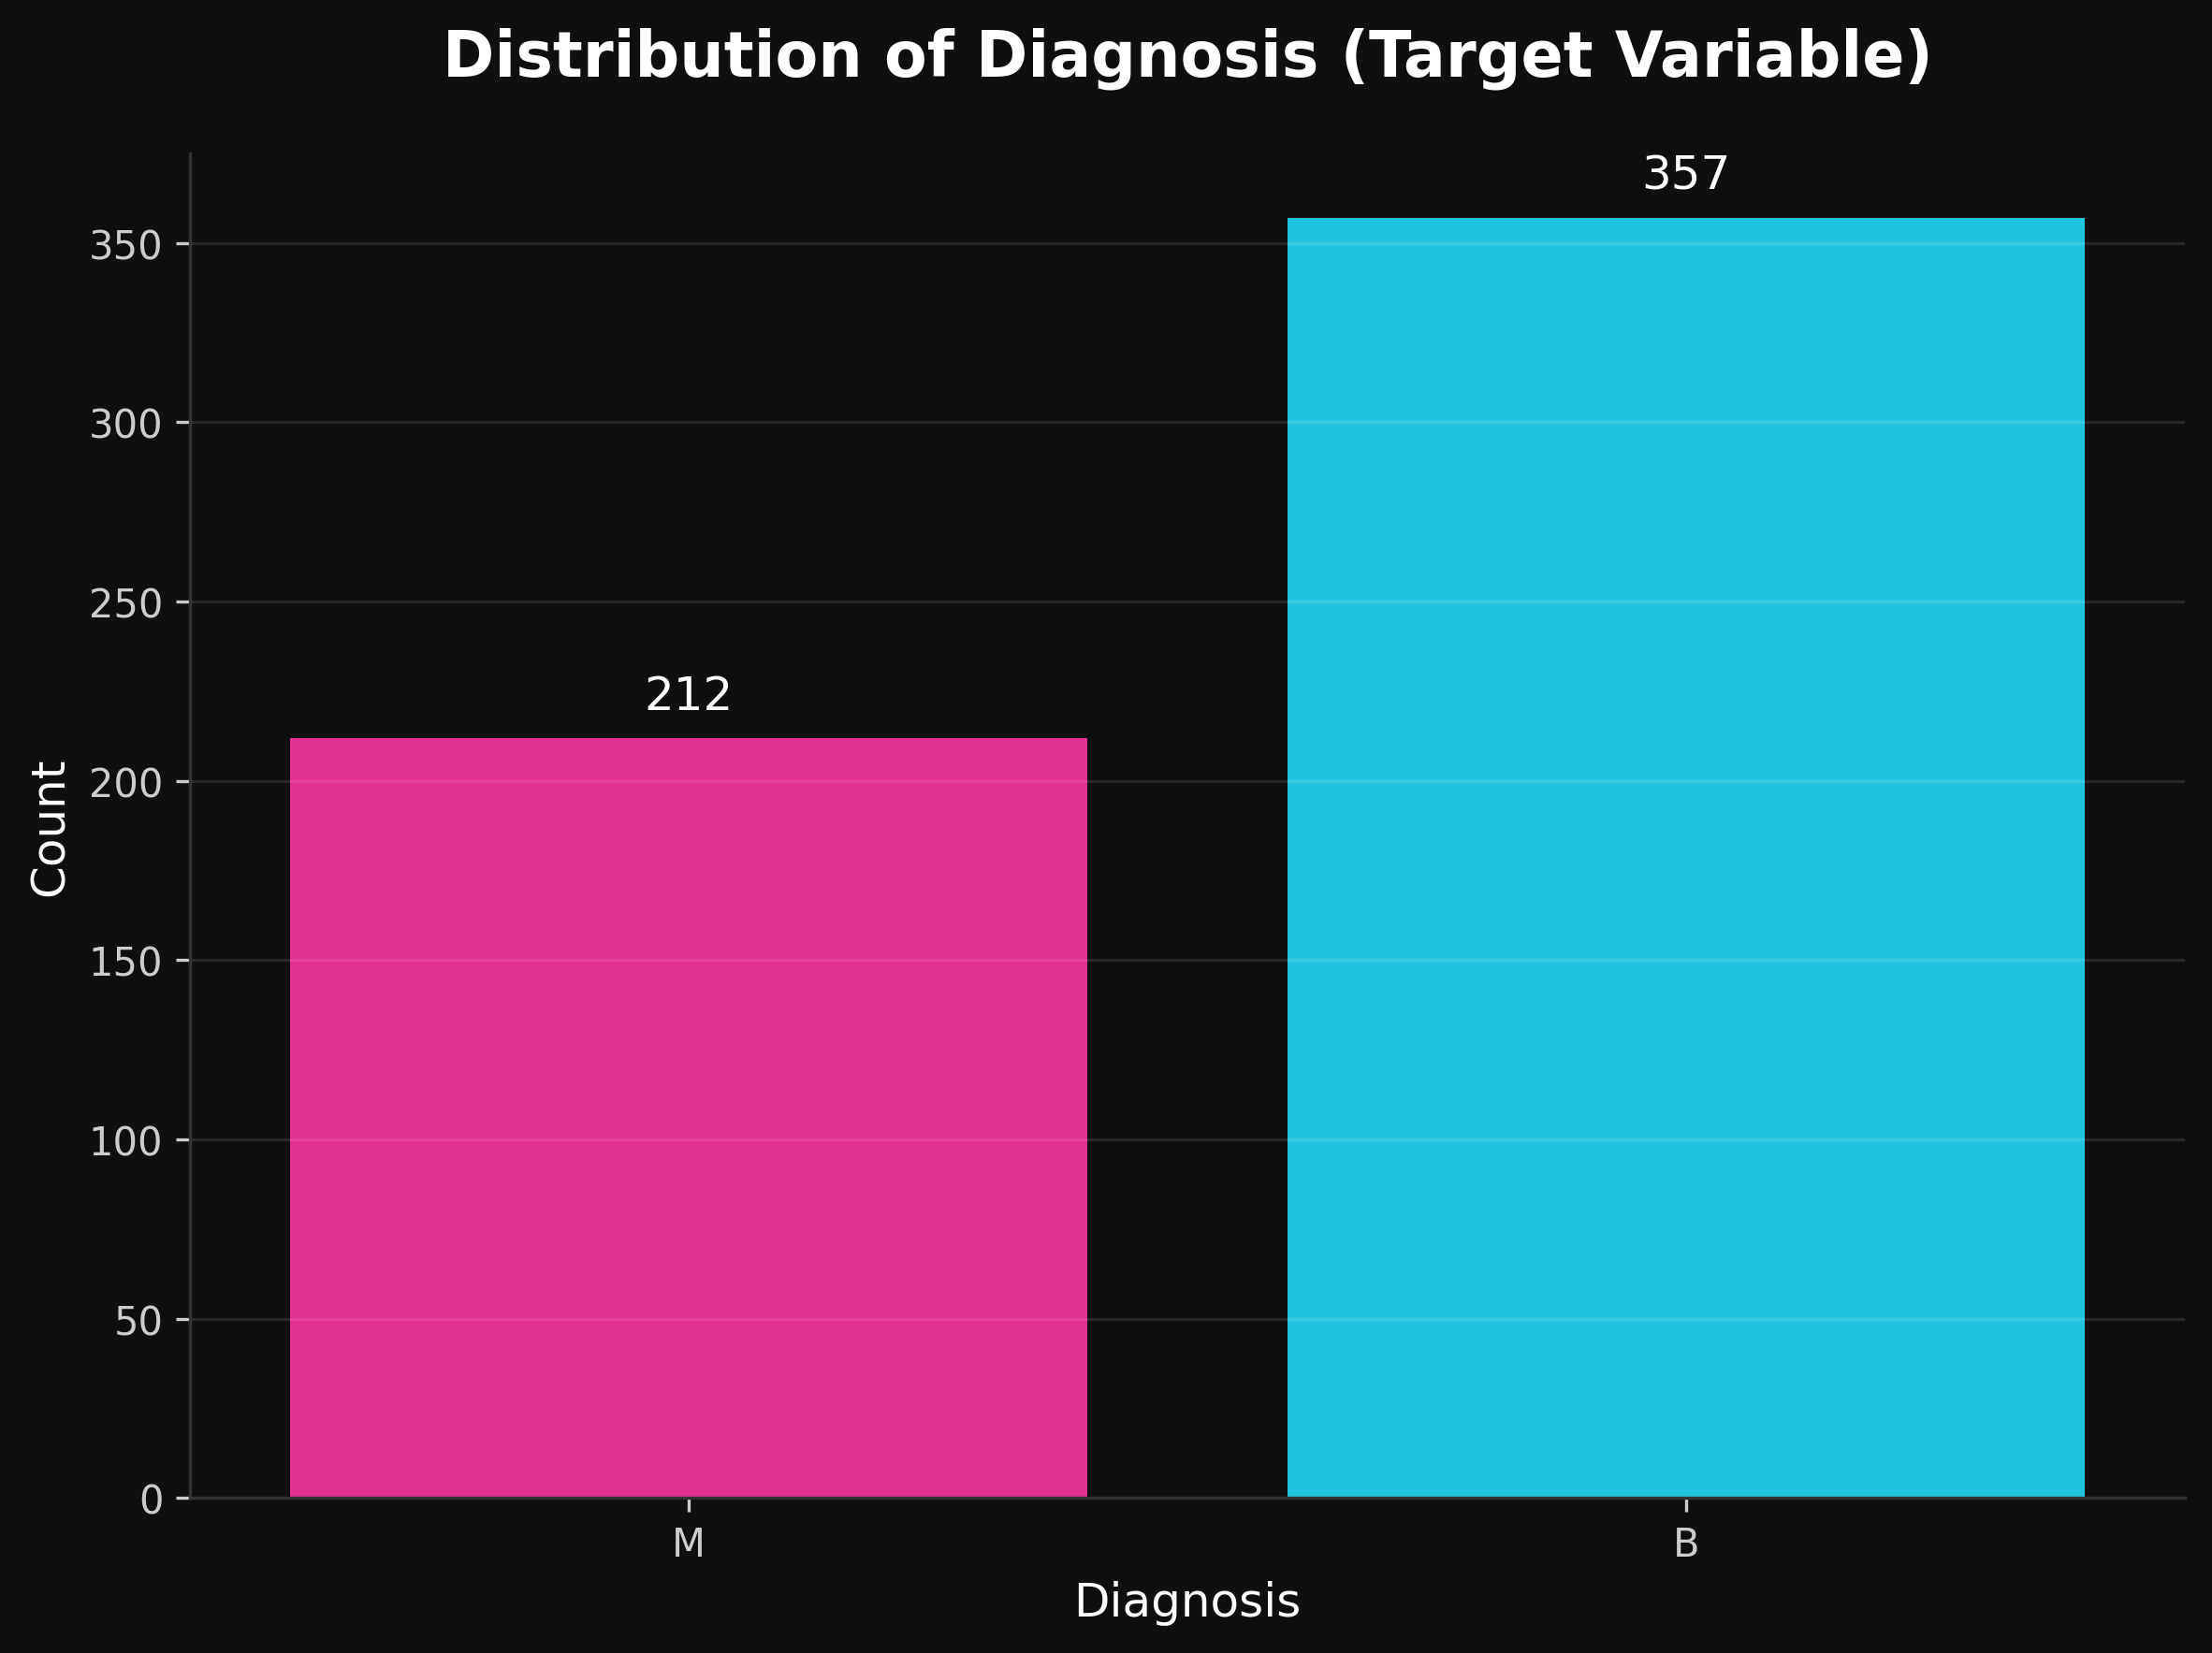
\includegraphics[width=0.7\textwidth]{images/wbcd_target_dist.png}
    \caption{Distribution of Diagnosis in WBCD Dataset}
    \label{fig:wbcd_target_dist}
\end{figure}

The majority of cases are Benign (Cyan), while Malignant cases (Pink) constitute approximately 37\% of the data. This imbalance necessitates the use of stratified sampling and specific evaluation metrics like F1-score and Sensitivity, rather than simple Accuracy.

\subsubsection{Feature Linearity and Correlation Analysis}
To identify the most predictive features, we analyzed the correlation of each feature with the target variable (encoded as Malignant=1).

\begin{figure}[H]
    \centering
    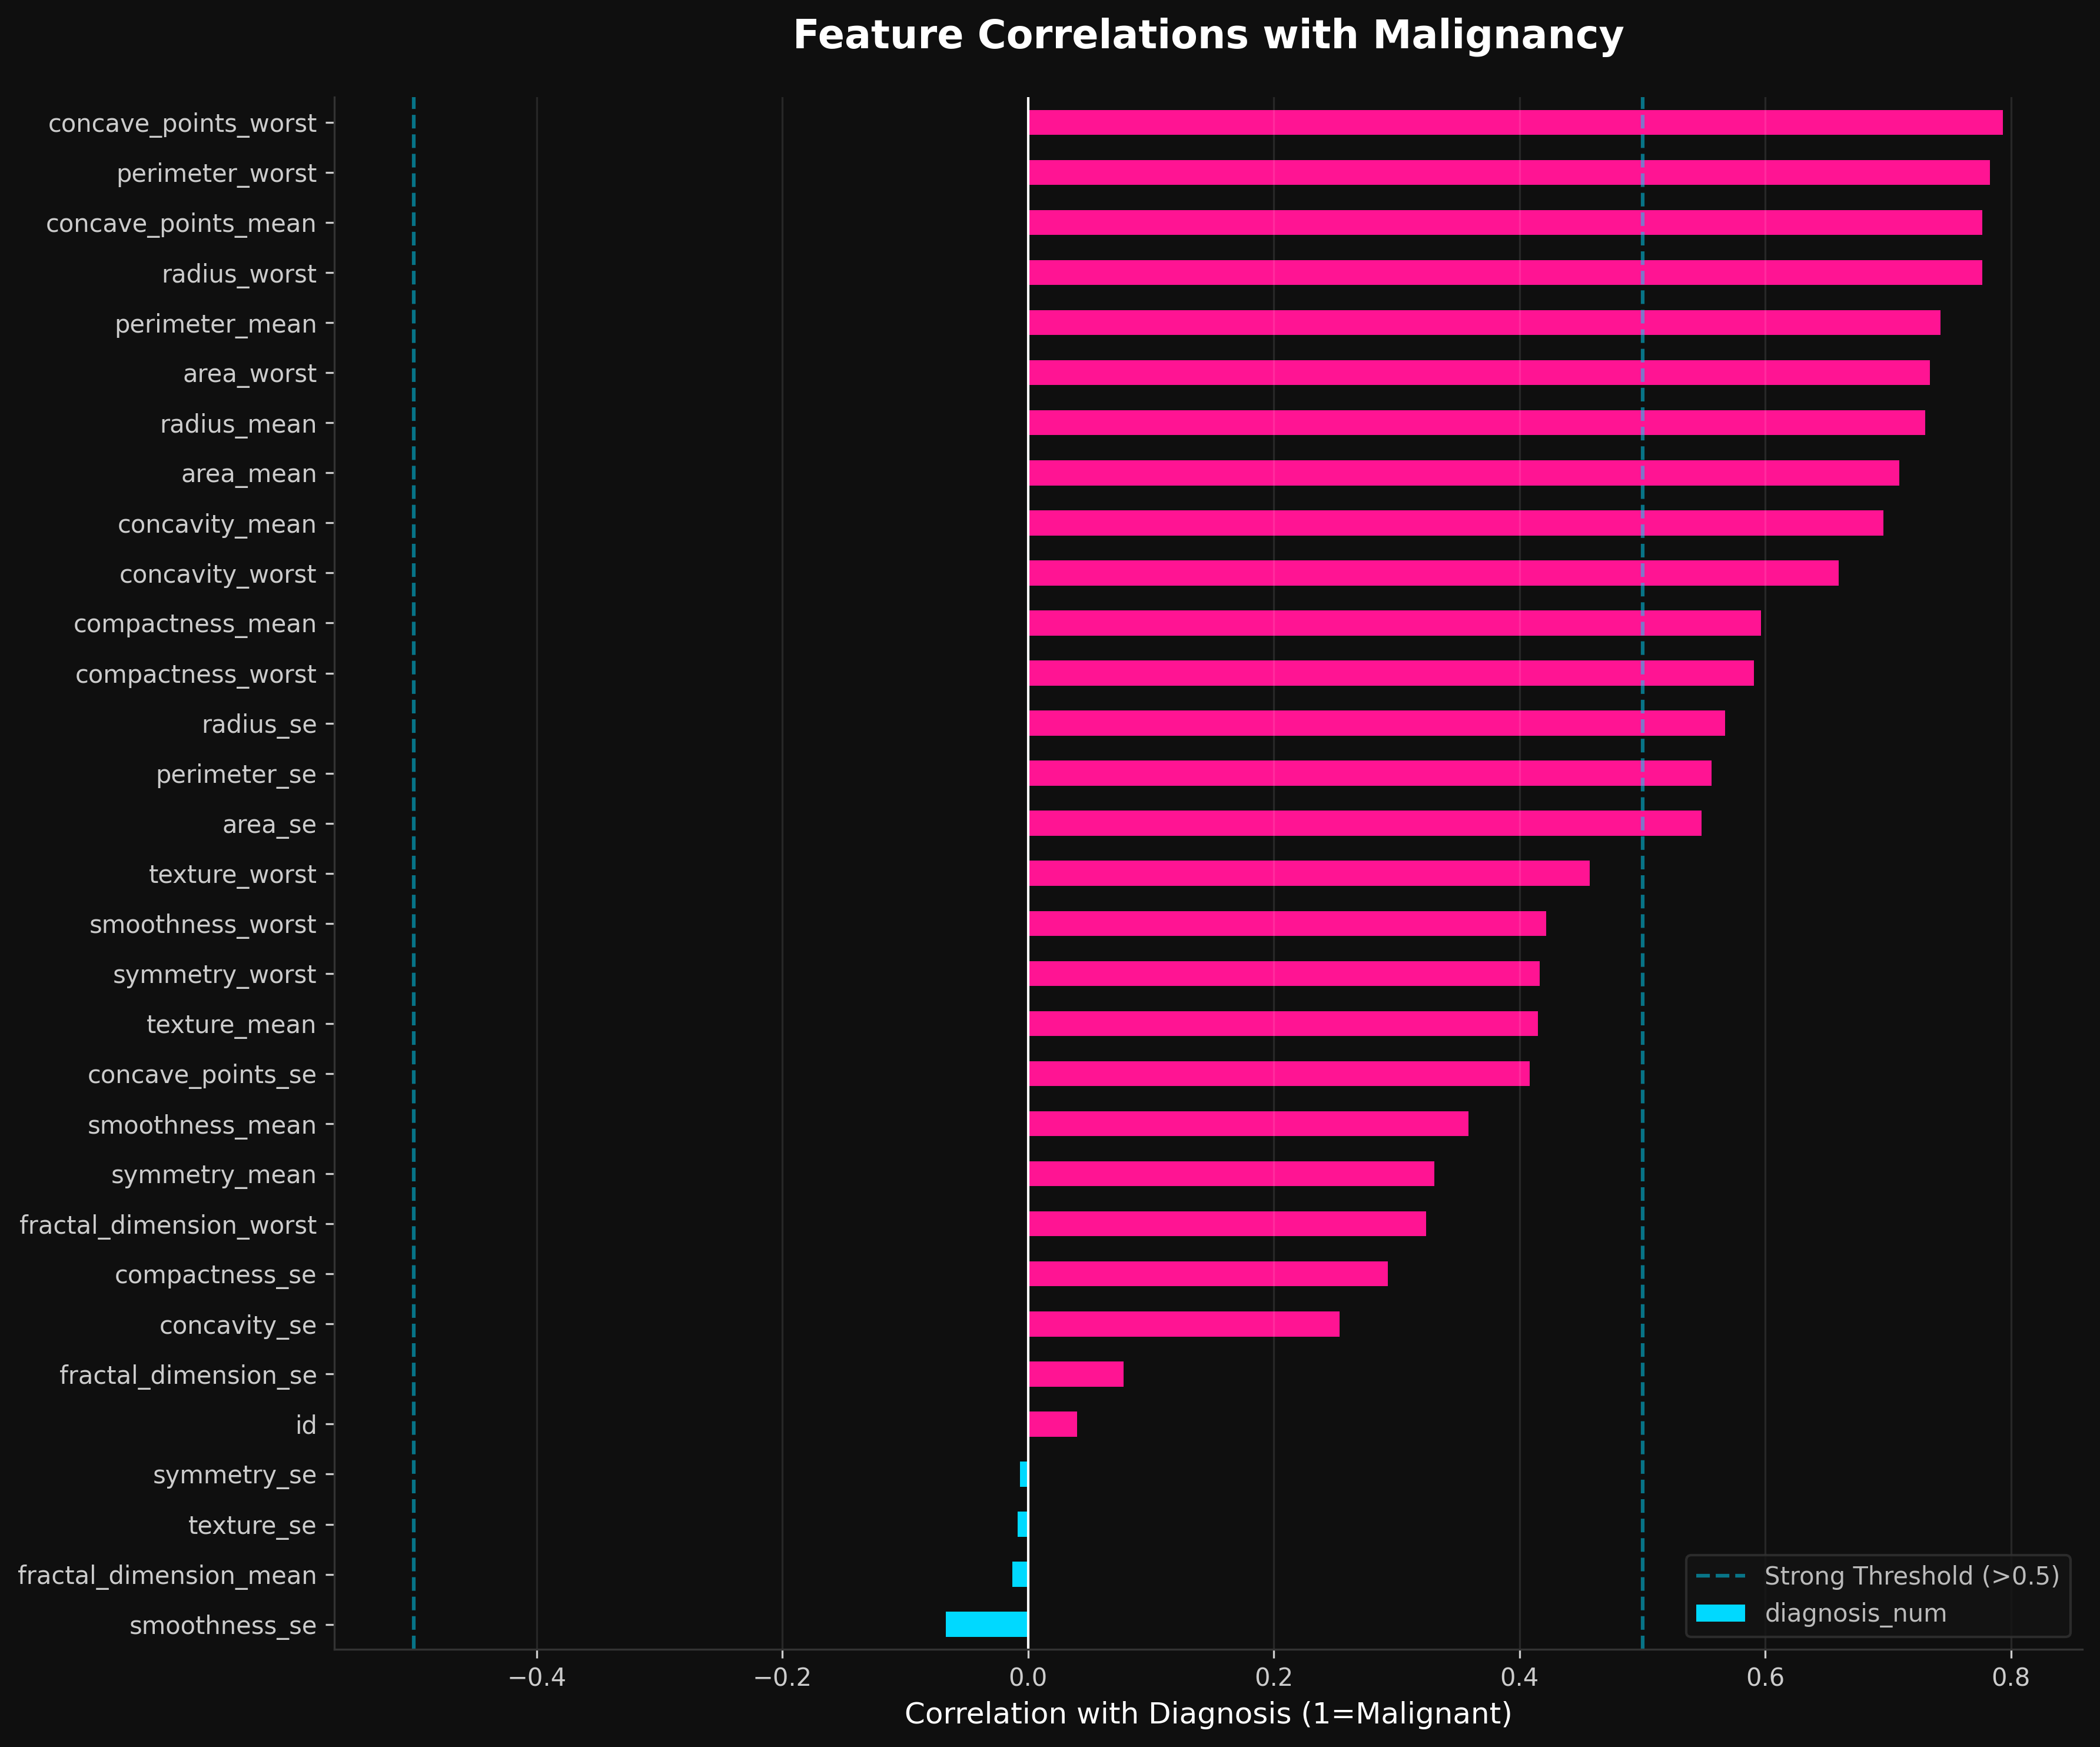
\includegraphics[width=0.6\textwidth]{images/wbcd_correlation_barh.png}
    \caption{Feature Correlations with Malignancy}
    \label{fig:wbcd_corr_barh}
\end{figure}

The horizontal bar chart highlights features with the strongest influence:
\begin{itemize}
    \item \textbf{Positive Correlation (Pink):} Features like \texttt{concave points\_worst}, \texttt{perimeter\_worst}, and \texttt{radius\_worst} show very strong positive correlation ($> 0.7$) with malignancy. Larger, more irregular nuclei are strong indicators of cancer.
    \item \textbf{Negative Correlation (Cyan):} Some texture and fractal dimension features show weaker or negative correlations.
\end{itemize}
High multicollinearity is also observed among geometric features (e.g., Radius, Perimeter, Area), suggesting that dimensionality reduction or regularization (e.g., L2 penalty) could be beneficial.

\subsection{METABRIC Exploratory Data Analysis}
The \textbf{Molecular Taxonomy of Breast Cancer International Consortium (METABRIC)} dataset was analyzed following a structured approach to understand the underlying distributions and relationships before modeling.

\subsubsection{Dataset Overview}
The METABRIC dataset serves as the foundation for the prognosis prediction tasks. It combines clinical attributes with detailed genomic profiles to enable multi-faceted patient evaluation.
\begin{itemize}
    \item \textbf{Instances:} 1,904 patients.
    \item \textbf{Features:} Clinical variables (e.g., Age, Tumor Size, Lymph Nodes) and genomic markers.
    \item \textbf{Objective:} To predict tumor aggressiveness, growth rate, and 6-month evolution status.
\end{itemize}

\subsubsection{Missing Value Analysis}
Data quality is critical for reliable regression modeling. The missing value analysis reveals a generally high-quality dataset, though some imputation is required.

\begin{figure}[H]
    \centering
    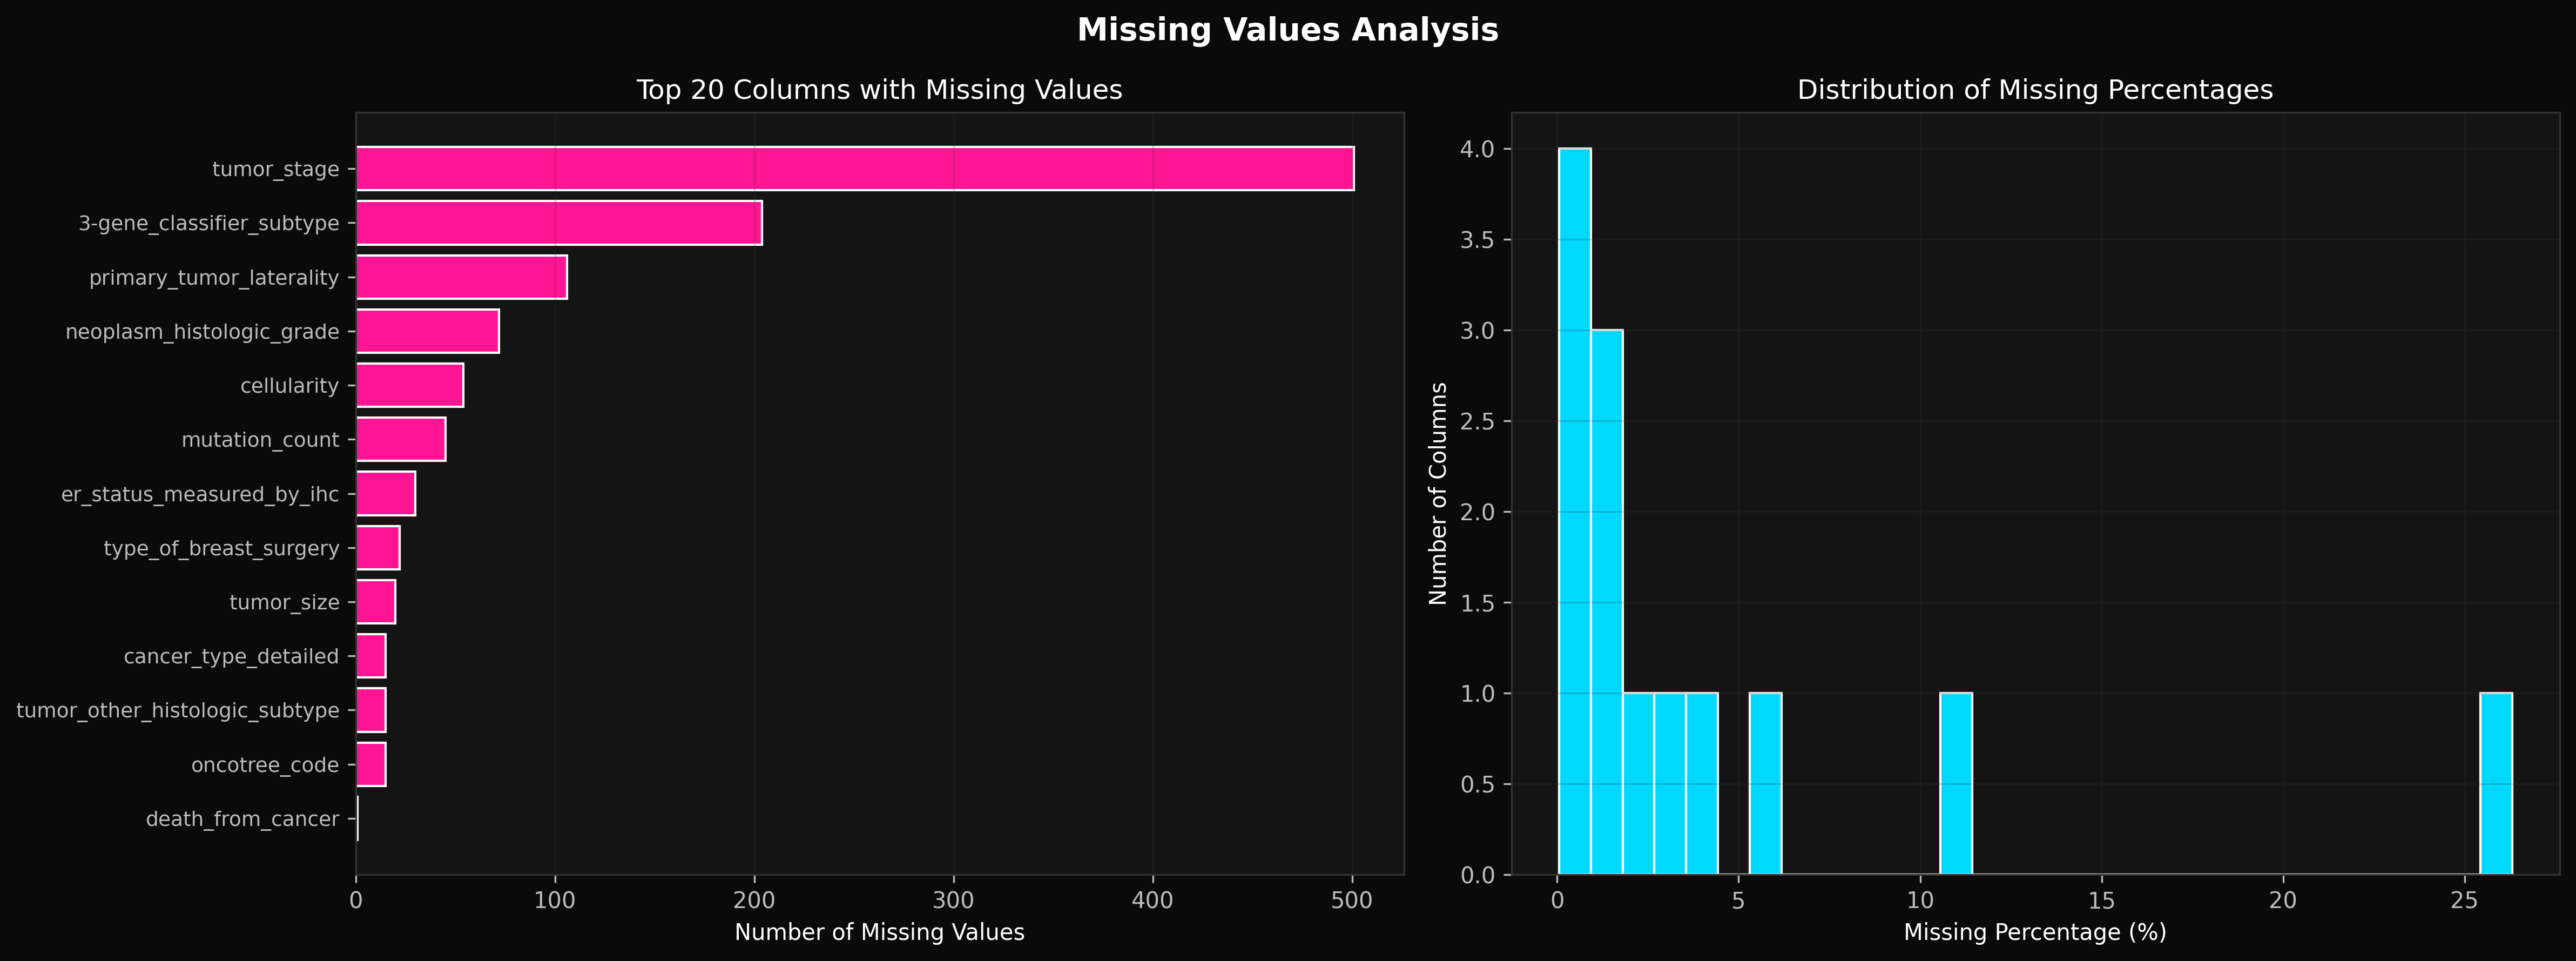
\includegraphics[width=\textwidth]{images/metabric_missing_values.png}
    \caption{Missing Value Analysis: Top Columns and Distribution}
    \label{fig:metabric_missing}
\end{figure}

The visualization highlights that while most columns are complete, specific clinical features (e.g., \texttt{tumor\_stage}, \texttt{tumor\_size}) contain missing entries that must be addressed during preprocessing.

\subsubsection{Clinical Variable Statistics}
Key statistical measures for the primary clinical features are summarized below.

\begin{table}[H]
\centering
\renewcommand{\arraystretch}{0.9}
\scalebox{0.92}{
\begin{tabular}{|l|c|c|c|c|}
\hline
\textbf{Feature} & \textbf{Mean} & \textbf{Std Dev} & \textbf{Min} & \textbf{Max} \\ \hline
age\_at\_diagnosis & 61.087 & 12.979 & 21.930 & 96.290 \\ \hline
tumor\_size & 25.075 & 10.780 & 1.000 & 49.500 \\ \hline
nottingham\_prognostic\_index & 4.033 & 1.144 & 1.000 & 6.360 \\ \hline
lymph\_nodes\_examined\_positive & 1.295 & 1.770 & 0.000 & 5.000 \\ \hline
mutation\_count & 5.681 & 4.012 & 1.000 & 80.000 \\ \hline
overall\_survival\_months & 125.121 & 76.334 & 0.000 & 355.200 \\ \hline
\end{tabular}
}
\caption{Descriptive Statistics for METABRIC Clinical Features}
\label{tab:metabric_stats}
\end{table}

\subsubsection{Numerical Variable Distribution}
The distributions of continuous variables provide insights into the patient population demographics and tumor characteristics.

\begin{figure}[H]
    \centering
    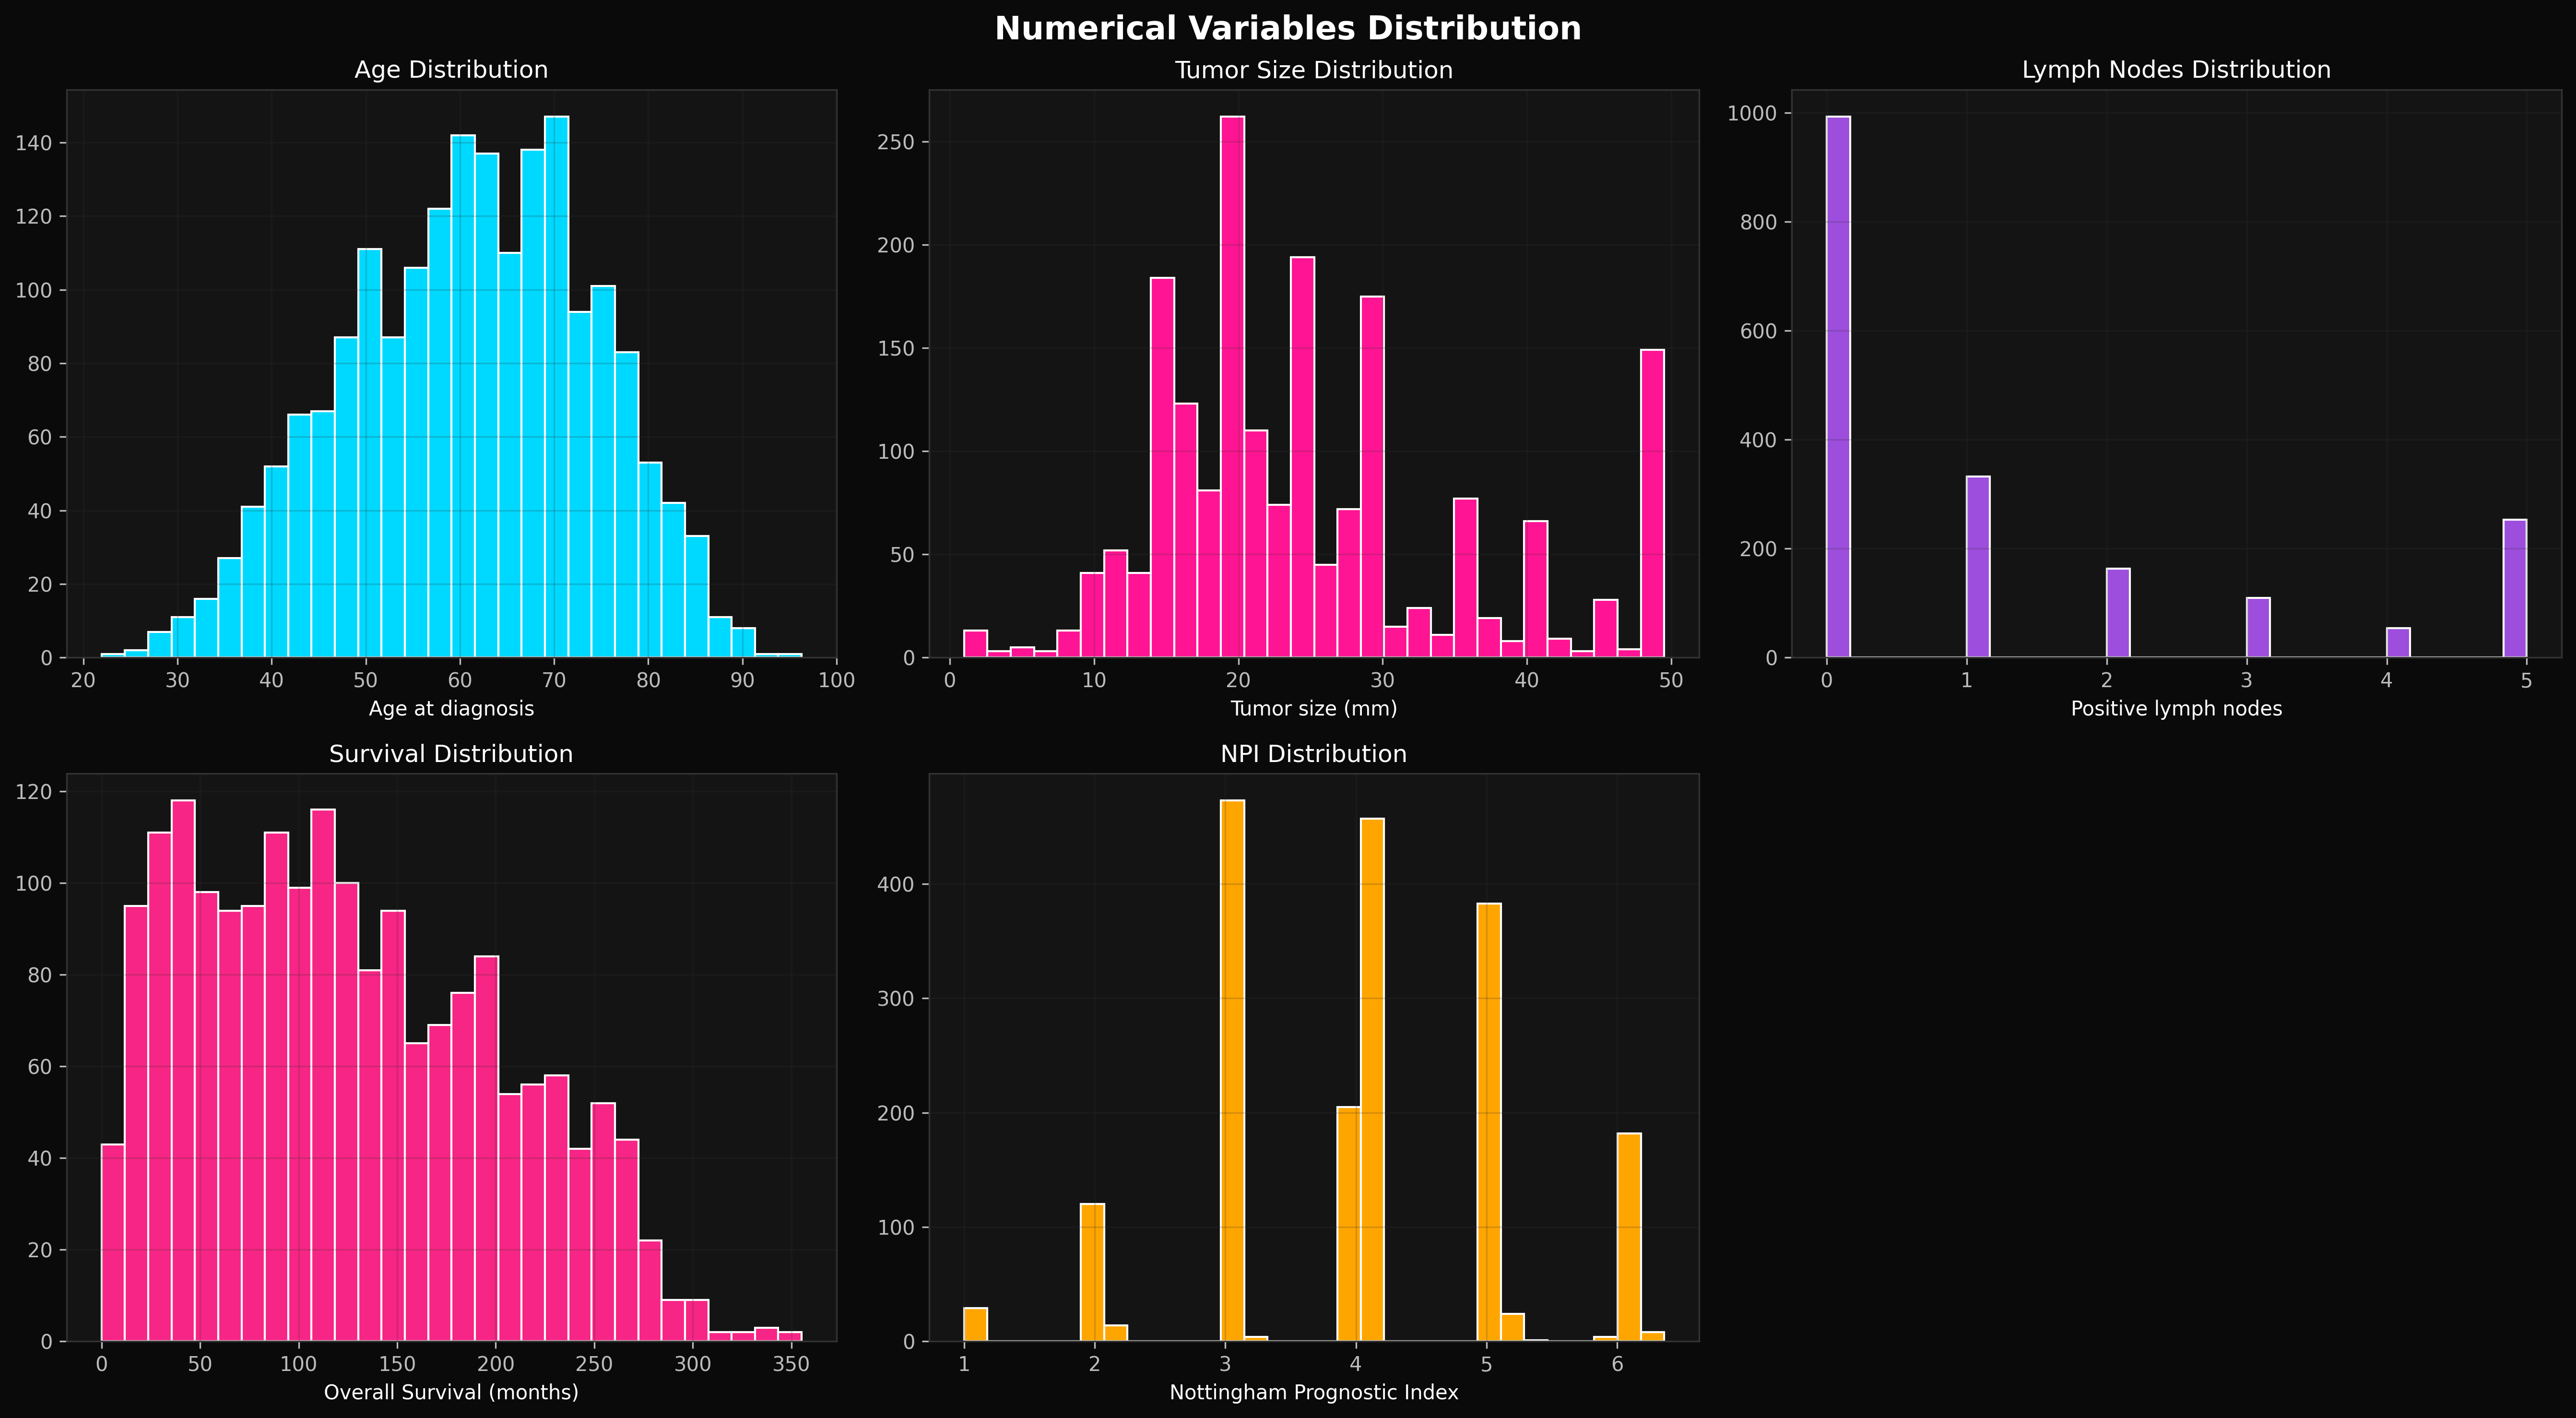
\includegraphics[width=\textwidth]{images/metabric_numerical_dist.png}
    \caption{Distribution of Numerical Clinical Variables}
    \label{fig:metabric_numerical}
\end{figure}

\begin{itemize}
    \item \textbf{Age:} The age distribution is roughly normal, centered around 60 years.
    \item \textbf{Tumor Size:} Shows a right-skewed distribution, indicating most tumors are detected at a smaller size.
    \item \textbf{Lymph Nodes:} Highly right-skewed, with most patients having few positive nodes.
    \item \textbf{Survival Months:} A wide distribution reflecting the variable nature of breast cancer prognosis.
\end{itemize}

\subsubsection{Categorical Variables Distribution}
Categorical features such as histologic grade and tumor stage are essential for risk stratification.

\begin{figure}[H]
    \centering
    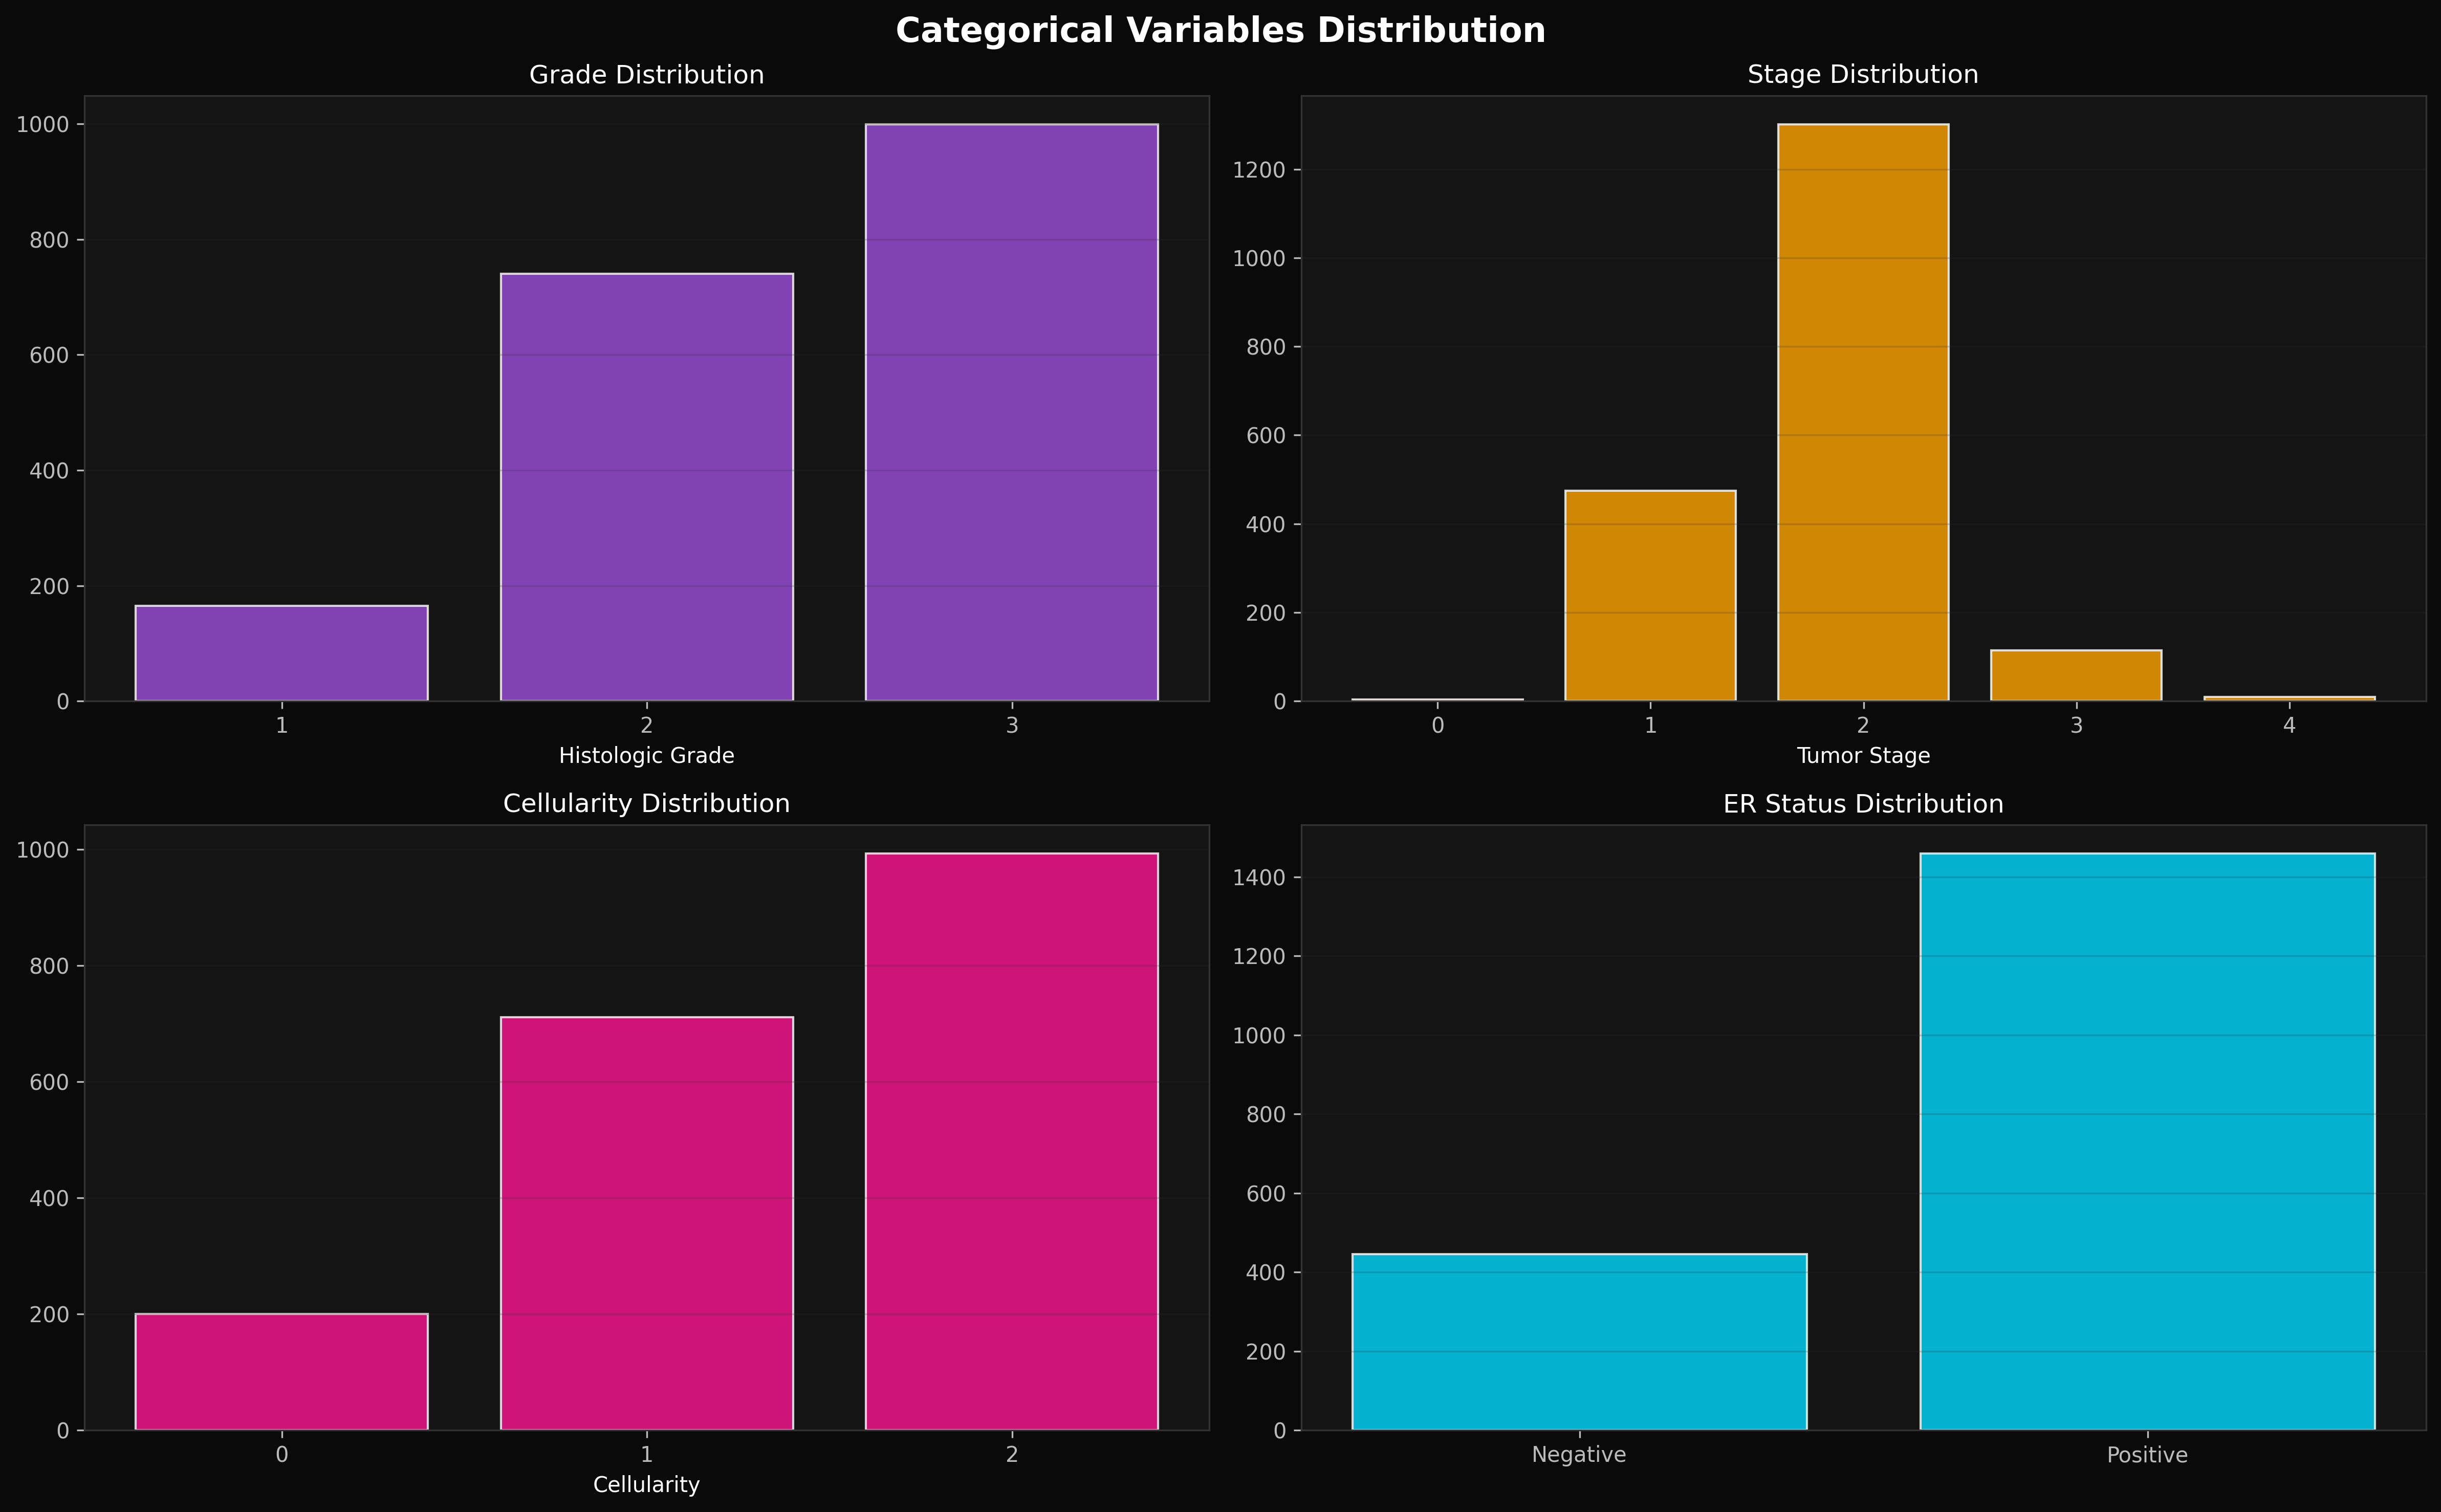
\includegraphics[width=0.7\textwidth]{images/metabric_categorical_dist.png}
    \caption{Distribution of Categorical Clinical Variables}
    \label{fig:metabric_categorical}
\end{figure}

The plots reveal the prevalence of different cancer grades and stages, which are direct inputs into the Aggressiveness Score calculation.

\subsubsection{Correlation Analysis}
To understand the interdependencies between clinical variables, a correlation matrix was generated.

\begin{figure}[H]
    \centering
    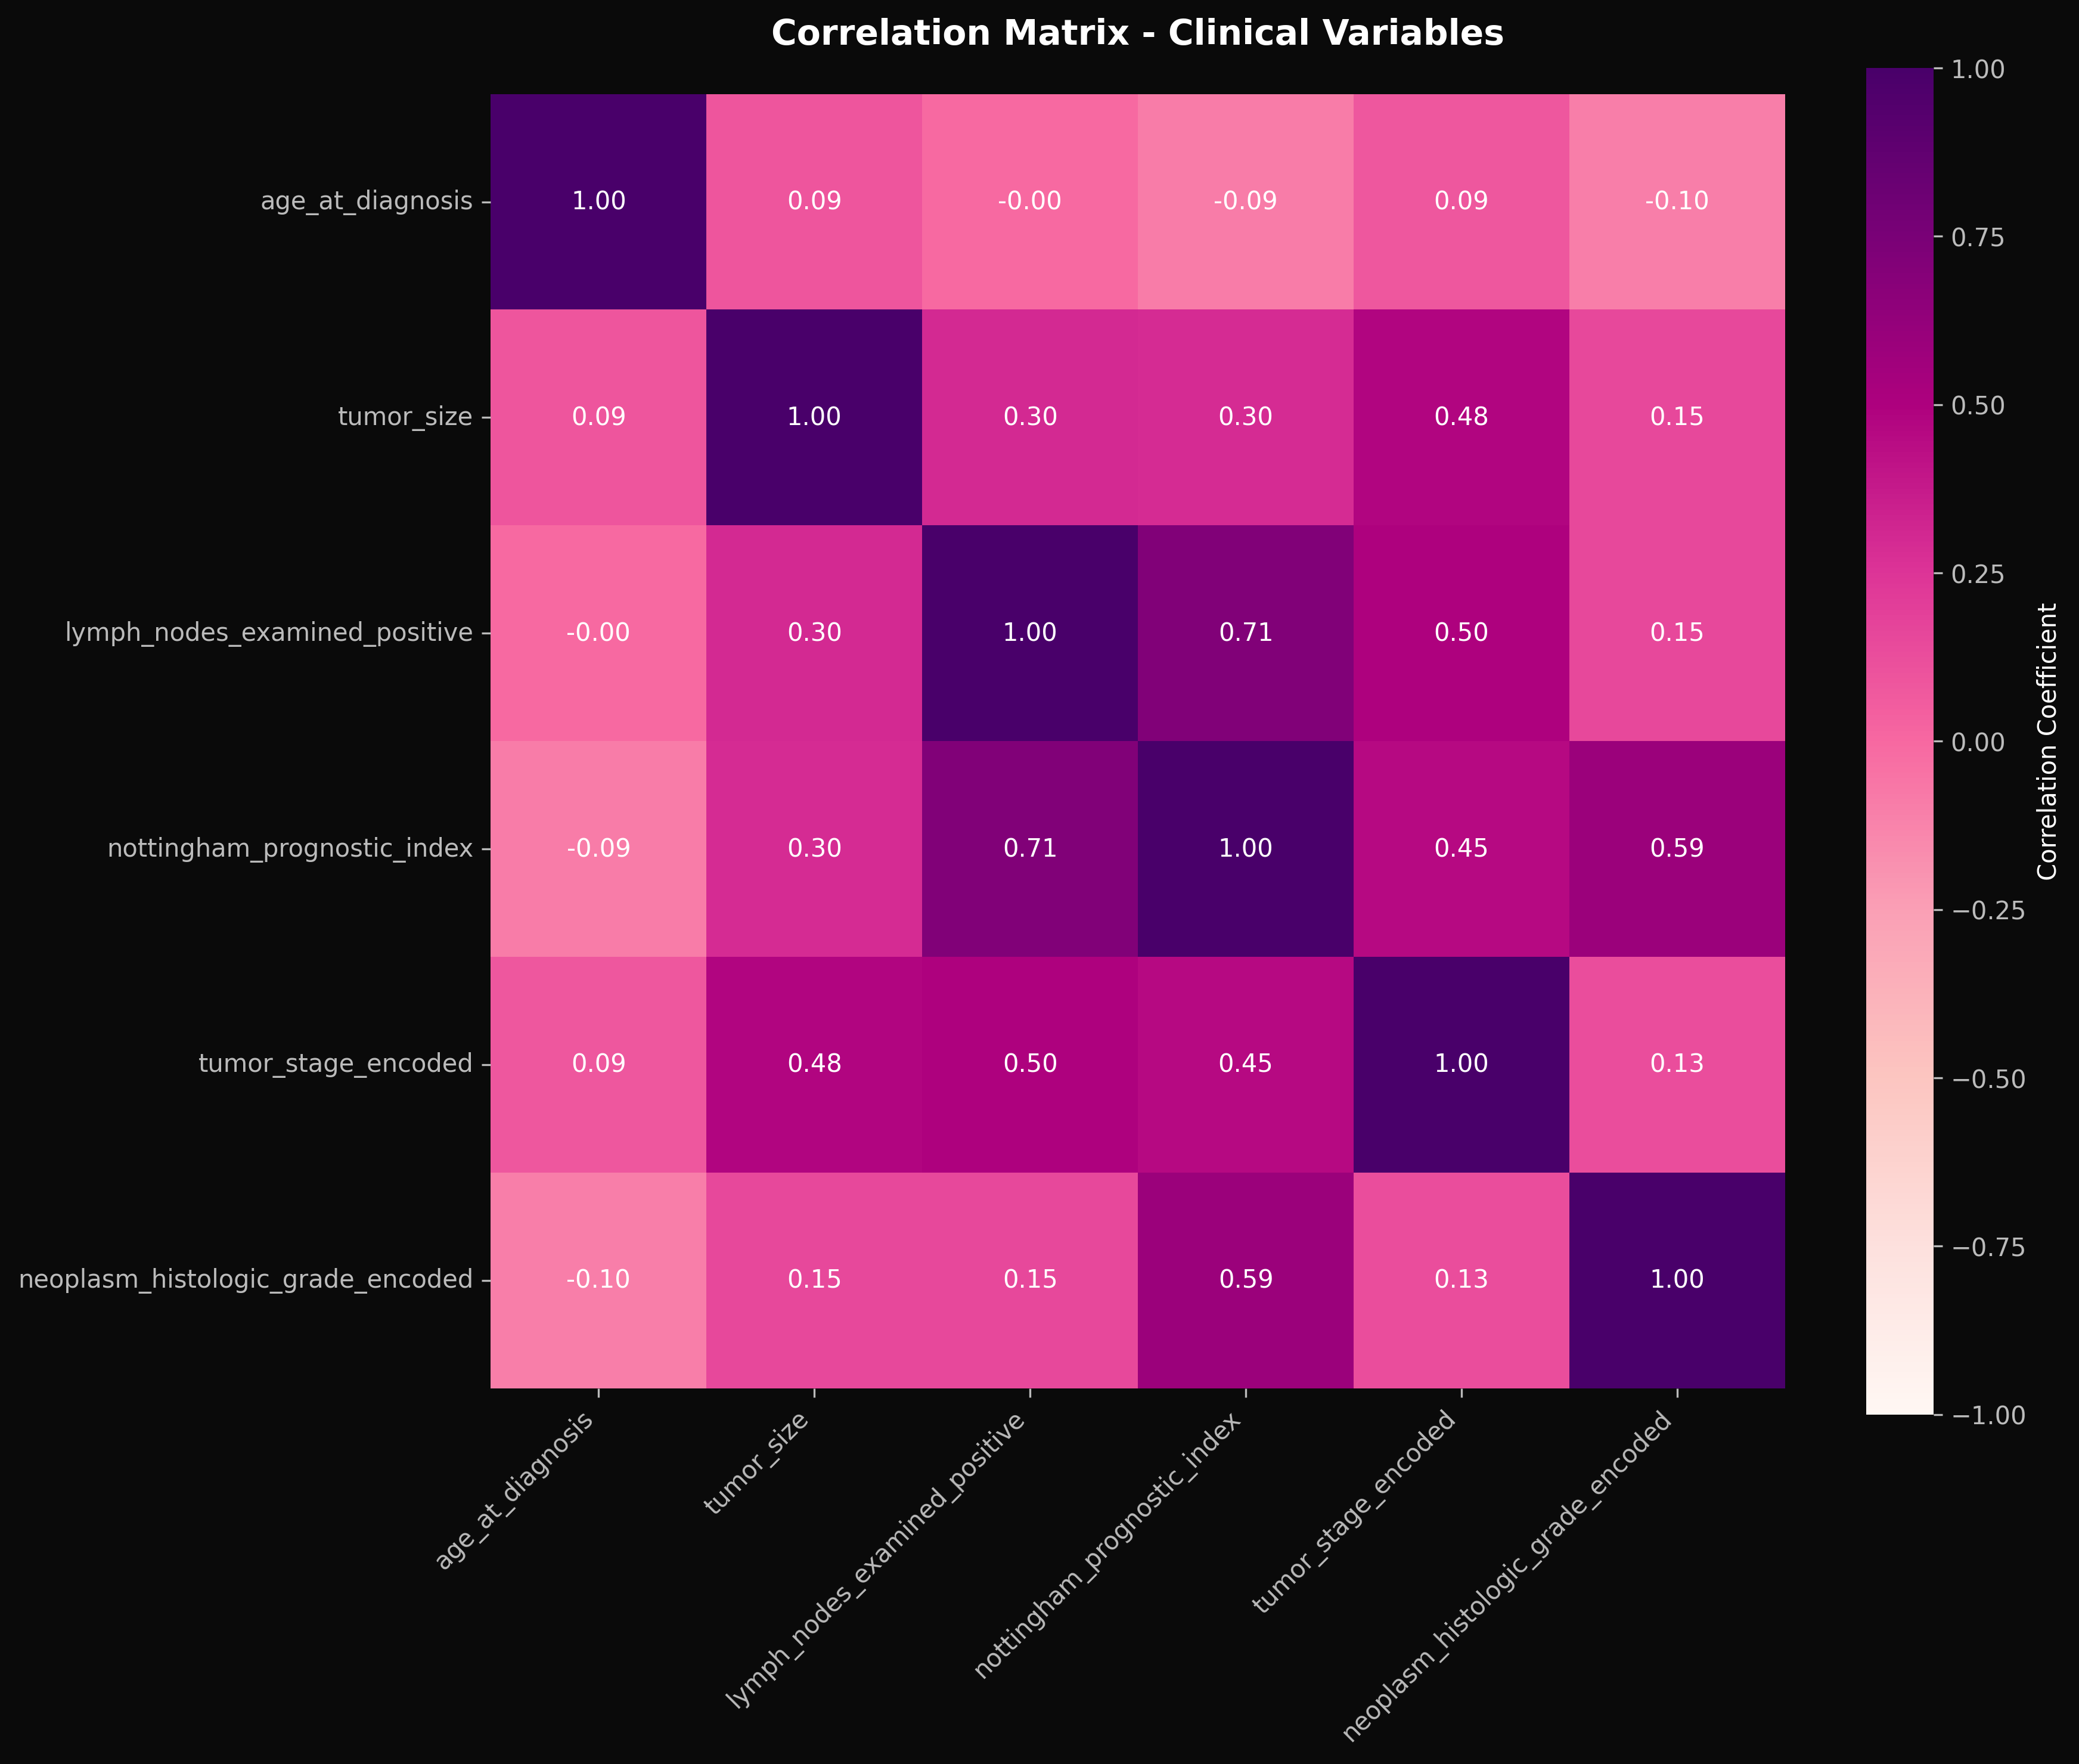
\includegraphics[width=0.5\textwidth]{images/metabric_correlation.png}
    \caption{Correlation Matrix of Clinical Variables}
    \label{fig:metabric_corr}
\end{figure}

\begin{itemize}
    \item \textbf{NPI \& Grade:} Strong positive correlation, as NPI is mathematically derived from grade.
    \item \textbf{Tumor Size \& Stage:} Positive correlation, as larger tumors typically correspond to advanced stages.
    \item \textbf{Nodes \& NPI:} Significant correlation, reinforcing the NPI as a composite measure of severity.
\end{itemize}

\chapter{Data Preprocessing and Cleaning}

Effective preprocessing is crucial for model performance, especially in medical datasets where noise and scale discrepancies can lead to critical prediction errors. The preprocessing workflow is divided into two distinct pipelines: one for the diagnosis task (WBCD) and one for the prognosis task (METABRIC).

\section{WBCD Data Preprocessing}
The preprocessing pipeline for the Wisconsin Breast Cancer Diagnosis (WBCD) dataset focuses on preparing the features for binary classification.

\subsection{Encoding Target Variable}
The target variable \texttt{diagnosis} initially consists of categorical labels: 'M' (Malignant) and 'B' (Benign). Since machine learning algorithms operate on numerical data, Label Encoding was applied to map these categories to binary values:
\begin{itemize}
    \item \textbf{Malignant (M)} $\rightarrow$ \textbf{1} (Positive Class)
    \item \textbf{Benign (B)} $\rightarrow$ \textbf{0} (Negative Class)
\end{itemize}
This encoding ensures that the model correctly identifies the presence of cancer as the positive case.

\subsection{Train-Test Split}
To assess the model's generalization capability, the dataset was split into independent training and testing subsets.
\begin{itemize}
    \item \textbf{Ratio:} 70\% of the data was allocated for training, and 30\% for testing.
    \item \textbf{Stratification:} A stratified split was employed to ensure that the proportion of Malignant and Benign cases remains consistent across both the training and testing sets. This is vital given the class imbalance observed in the EDA phase.
\end{itemize}

\subsection{Standardization}
The WBCD dataset features vary significantly in magnitude (e.g., \texttt{area\_mean} $\approx$ 650 vs. \texttt{smoothness\_mean} $\approx$ 0.1). Distance-based algorithms (like KNN and SVM) and gradient-descent-based models are sensitive to these scale differences.

To address this, \textbf{StandardScaler} was used to normalize the features. This technique rescales the distribution of values so that the mean of observed values is 0 and the standard deviation is 1. The mathematical equation applied is:

\begin{equation}
    z = \frac{x - \mu}{\sigma}
\end{equation}

Where:
\begin{itemize}
    \item $z$ is the standardized value (z-score).
    \item $x$ is the original feature value.
    \item $\mu$ is the mean of the feature in the training set.
    \item $\sigma$ is the standard deviation of the feature in the training set.
\end{itemize}
Note that the scaler is fit only on the training set and then used to transform the test set to prevent data leakage.

\section{METABRIC Data Preprocessing}
For the prognosis task, the METABRIC dataset required a more complex preprocessing pipeline due to its high dimensionality and mixed data types. The process was divided into eight key stages:

\subsection{Column Selection}
The original dataset contained 693 columns. To reduce noise and focus on clinically relevant features, the dataset was reduced to 23 core columns, including patient demographics, tumor characteristics, and genetic mutations.

(See Appendix \ref{app:feature_selection} for implementation details).

\subsection{Data Imputation}
Missing values were handled based on variable type to preserve distribution characteristics:
\begin{itemize}
    \item \textbf{Numerical Variables:} Missing values were imputed using the \textbf{median} (robust to outliers).
    \item \textbf{Categorical Variables:} Missing values were imputed using the \textbf{mode} (most frequent category).
    \item \textbf{Mutation Counts:} Missing values were filled with 0, assuming no mutation was detected.
\end{itemize}
(See Appendix \ref{app:imputation} for implementation details).

\subsection{Outlier Detection and Treatment}
Outliers in numerical features (e.g., \texttt{tumor\_size}) were detected using the Interquartile Range (IQR) method. Values exceeding the upper bound (Q3 + 1.5 * IQR) were capped at the 95th percentile to prevent them from skewing the model. (See Appendix \ref{app:outliers} for implementation details).

\subsection{Categorical Encoding}
Categorical variables were encoded to be machine-readable:
\begin{itemize}
    \item \textbf{Binary Encoding:} Variables like \texttt{her2\_status} were mapped to 0 (Negative) and 1 (Positive).
    \item \textbf{Ordinal Encoding:} \texttt{cellularity} was mapped to ordered integers (Low=1, Moderate=2, High=3).
    \item \textbf{Survival Status:} 'Living' $\rightarrow$ 0, 'Died of Disease' $\rightarrow$ 1, 'Died of Other Causes' $\rightarrow$ 0.
\end{itemize}

\subsection{Feature Engineering}
New features were derived to capture complex biological interactions:
\begin{itemize}
    \item \textbf{Hormone Receptor Score:} Sum of ER and PR status.
    \item \textbf{Triple Negative:} Flag identifying patients negative for ER, PR, and HER2.
    \item \textbf{Grade-Stage Interaction:} Product of tumor grade and stage.
    \item \textbf{High Risk Score:} Binary flag if NPI > 5.4.
\end{itemize}
(See Appendix \ref{app:feature_eng} for implementation details).

\subsection{Target Variable Creation}
To predict disease progression, a composite \textbf{Aggressiveness Score} was calculated based on grade, stage, lymph nodes, and NPI. This score was then used to define the \texttt{evolution\_6m} target. (See Appendix \ref{app:target_creation} for implementation details).

\subsection{Train-Test Split}
The dataset was split into training (80\%) and testing (20\%) sets. Crucially, the split was \textbf{stratified by} \texttt{evolution\_6m} to ensure that all risk categories (Low, Medium, High) were equally represented in both sets.

\subsection{Feature Standardization}
Finally, all numerical features were standardized using \textbf{StandardScaler} to ensure that features like \texttt{tumor\_size} and \texttt{age} contributed equally to the model, regardless of their original units.

\chapter{Modeling}

The modeling phase is divided into three Business Objectives (BO), each addressing a specific aspect of breast cancer diagnosis and prognosis. This chapter details the mathematical formulations, hyperparameter choices, and business ("métier") rationale for the selected models.

\section{Business Objective 1: Tumor Classification (Diagnostic)}
The primary goal of BO1 is to accurately classify tumor samples as \textbf{Benign} or \textbf{Malignant} based on cytological features. We developed and optimized three distinct architectures: a Hybrid GRU-SVM model, Softmax Regression, and an SGD-optimized SVM.

\subsection{Model 1: Hybrid GRU-SVM}
To further improve classification performance, particularly in minimizing False Negatives, we implemented a hybrid architecture combining Deep Learning for feature extraction with a traditional SVM classifier.

\subsubsection{Concept}
Standard models treat features as independent or linearly related. This hybrid model uses a \textbf{Gated Recurrent Unit (GRU)} to learn complex, non-linear latent representations of the data, which are then fed into an \textbf{SVM} for the final decision. This leverages the feature learning capability of Neural Networks and the max-margin robustness of SVMs.

\subsubsection{Mathematical Formulation}
\begin{itemize}
    \item \textbf{Feature Reshaping:} The 30 input features are reshaped into a sequence $X \in \mathbb{R}^{5 \times 6}$ (5 timesteps, 6 features per step) to simulate sequential dependency.
    \item \textbf{Feature Extraction (GRU):} The GRU computes a hidden state $h_t$ at each step:
    \[ z_t = \sigma(W_z x_t + U_z h_{t-1}) \]
    \[ r_t = \sigma(W_r x_t + U_r h_{t-1}) \]
    \[ \tilde{h}_t = \tanh(W_h x_t + U_h (r_t \odot h_{t-1})) \]
    \[ h_t = (1 - z_t) \odot h_{t-1} + z_t \odot \tilde{h}_t \]
    The final state is projected to a latent space $L$ via a Dense layer with ReLU activation:
    \[ L = \text{ReLU}(W_L h_T + b_L) \]
    \item \textbf{Classification (SVM):} The latent vector $L$ serves as input to the SVM:
    \[ f(L) = \text{sign}\left(\sum_{i} \alpha_i y_i K(L_i, L) + b\right) \]
\end{itemize}

\subsubsection{Hyperparameter Choice}
\begin{itemize}
    \item \textbf{GRU Structure:} 128 Units, Dropout = 0.5 to prevent overfitting.
    \item \textbf{Learning Rate:} 0.001 for the GRU pre-training.
    \item \textbf{SVM Classifier:} Linear Kernel with a calibrated threshold of 0.25.
\end{itemize}

\subsubsection{Métier Rationale}
\begin{itemize}
    \item \textbf{Latent Feature Discovery:} The GRU acts as a sophisticated "filter," transforming raw cytological measurements into a more separable "latent" representation. This helps in distinguishing cases that look similar in the original space but are biologically different.
    \item \textbf{Sensitivity Focus:} By explicitly monitoring "Missed Cases" (False Negatives), this complex architecture aims to capture subtle patterns of malignancy that simpler linear models might miss, providing a "safety net" for the diagnostic process.
\end{itemize}

\subsection{Model 2: Softmax Regression (Logistic Regression)}
Softmax Regression (or Logistic Regression for binary tasks) models the probability that a sample belongs to the Malignant class.

\subsubsection{Mathematical Formulation}
The hypothesis function applies the sigmoid activation to the linear output:
\begin{equation}
    P(y=1|X) = \sigma(z) = \frac{1}{1 + e^{-(\theta^T X + b)}}
\end{equation}
The model minimizes the Log-Loss (Cross-Entropy) cost function with L2 regularization:
\begin{equation}
    J(\theta) = - \frac{1}{m} \sum_{i=1}^{m} [y^{(i)}\log(\hat{y}^{(i)}) + (1-y^{(i)})\log(1-\hat{y}^{(i)})] + \frac{1}{C} ||\theta||^2
\end{equation}

\subsubsection{Hyperparameter Choice}
We performed a Grid Search to identify the best configuration:
\begin{itemize}
    \item \textbf{Solver:} 'lbfgs' (Limited-memory BFGS) for efficient convergence on small datasets.
    \item \textbf{Regularization (C):} $C=10.0$. A higher $C$ implies weaker regularization, allowing the model to fit the decision boundary more closely to the training data, which is appropriate given the high dimensionality (30 features) relative to sample size.
    \item \textbf{Max Iterations:} 3000 to ensure convergence.
    \item \textbf{Decision Threshold:} $0.477$. This threshold was calibrated to optimize the Sensitivity/Specificity balance.
\end{itemize}

\subsubsection{Métier Rationale}
\begin{itemize}
    \item \textbf{Probabilistic Output:} Unlike simple linear classifiers, this model provides a calibrated probability score. A probability of 99\% vs 51\% allows oncologists to gauge the certainty of the diagnosis.
    \item \textbf{Threshold Calibration:} The threshold was lowered from the default 0.5 to 0.477. In a medical context, this slight bias towards the positive class (Malignant) acts as a safety buffer to reduce False Negatives.
\end{itemize}

\subsection{Model 3: SGD-SVM (Stochastic Gradient Descent)}
The third model employs a Support Vector Machine optimized via Stochastic Gradient Descent (SGD), designed for efficiency and fine-grained control over the learning process.

\subsubsection{Mathematical Formulation}
The model minimizes the regularized Hinge Loss function:
\begin{equation}
    J(w,b) = \frac{1}{n} \sum_{i=1}^{n} L(y_i, f(x_i)) + \alpha R(w)
\end{equation}
where $L$ is the Hinge Loss:
\begin{equation}
    L(y, f(x)) = \max(0, 1 - y(w \cdot x + b))
\end{equation}
The weights are updated iteratively:
\begin{equation}
    w \leftarrow w - \eta \left( \alpha w - \mathbb{I}[y_i(w \cdot x_i + b) < 1] y_i x_i \right)
\end{equation}

\subsubsection{Hyperparameter Choice}
\begin{itemize}
    \item \textbf{Loss Function:} 'hinge' (Standard SVM loss).
    \item \textbf{Penalty:} 'l2' (Ridge regularization).
    \item \textbf{Alpha (Regularization):} Dynamic $\alpha = \frac{1}{5 \times n\_samples}$. This dynamic setting scales regularization with dataset size.
    \item \textbf{Class Weight:} 'balanced'. This automatically adjusts weights inversely proportional to class frequencies, addressing the natural imbalance between Benign and Malignant cases.
    \item \textbf{Learning Rate:} Constant with $\eta_0 = 0.001$.
\end{itemize}

\subsubsection{Métier Rationale}
\begin{itemize}
    \item \textbf{Imbalance Handling:} The \texttt{class\_weight='balanced'} parameter is crucial in oncology, where malignant cases might be fewer than benign ones (or vice versa). It ensures the model doesn't bias towards the majority class.
    \item \textbf{Dynamic Regularization:} The dynamic alpha allows the model to adapt its complexity control based on the sample size, providing a robust solution that scales well if more patient data is collected over time.
\end{itemize}

\section{Business Objective 2: Intelligent Triage \& Resource Allocation}
The second objective addresses the operational bottleneck in radiology departments. We designed an AI-powered triage system to prioritize patient cases based on the predicted probability of malignancy, moving from a "First-In-First-Out" workflow to a Risk-Based Queue.

\subsection{Step 1: Probability Calibration}
To enable granular risk assessment, we require not just a binary label (0/1) but a calibrated probability score $P(y=1|X) \in [0, 1]$.

\subsubsection{Selected Engine}
We utilized the \textbf{SGD-SVM (Calibrated)} model as the core scoring engine. This choice is grounded in the model evaluation and comparison detailed in the next section. Although SVMs typically output a non-probabilistic decision function, we applied \textbf{Platt Scaling (Sigmoid Calibration)} to map the distance from the hyperplane to a probability distribution.

\begin{itemize}
    \item \textbf{Input:} 30 Standardized Nuclei Features.
    \item \textbf{Calibration Method:} Sigmoid function fitting on the validation set.
    \item \textbf{Output:} A continuous risk score where 0\% indicates high certainty of benignity and 100\% indicates high certainty of malignancy.
\end{itemize}

\subsection{Step 2: Explainability (XAI)}
Trust is the primary barrier to AI adoption in healthcare. To bridge this gap, we implemented a dual-layer explainability framework.

\subsubsection{Global Interpretability (Top Drivers)}
We analyzed the model's coefficients to identify which morphological features most strongly influence the cancer prediction. This global explainability was achieved by analyzing the \textbf{Feature Coefficients} from the trained SGD-SVM model.

Figure \ref{fig:feature_importance} visualizes the top drivers, separating "Malignant Drivers" (Positive Coefficients, Red) and "Benign Drivers" (Negative Coefficients, Blue).

\begin{figure}[h]
    \centering
    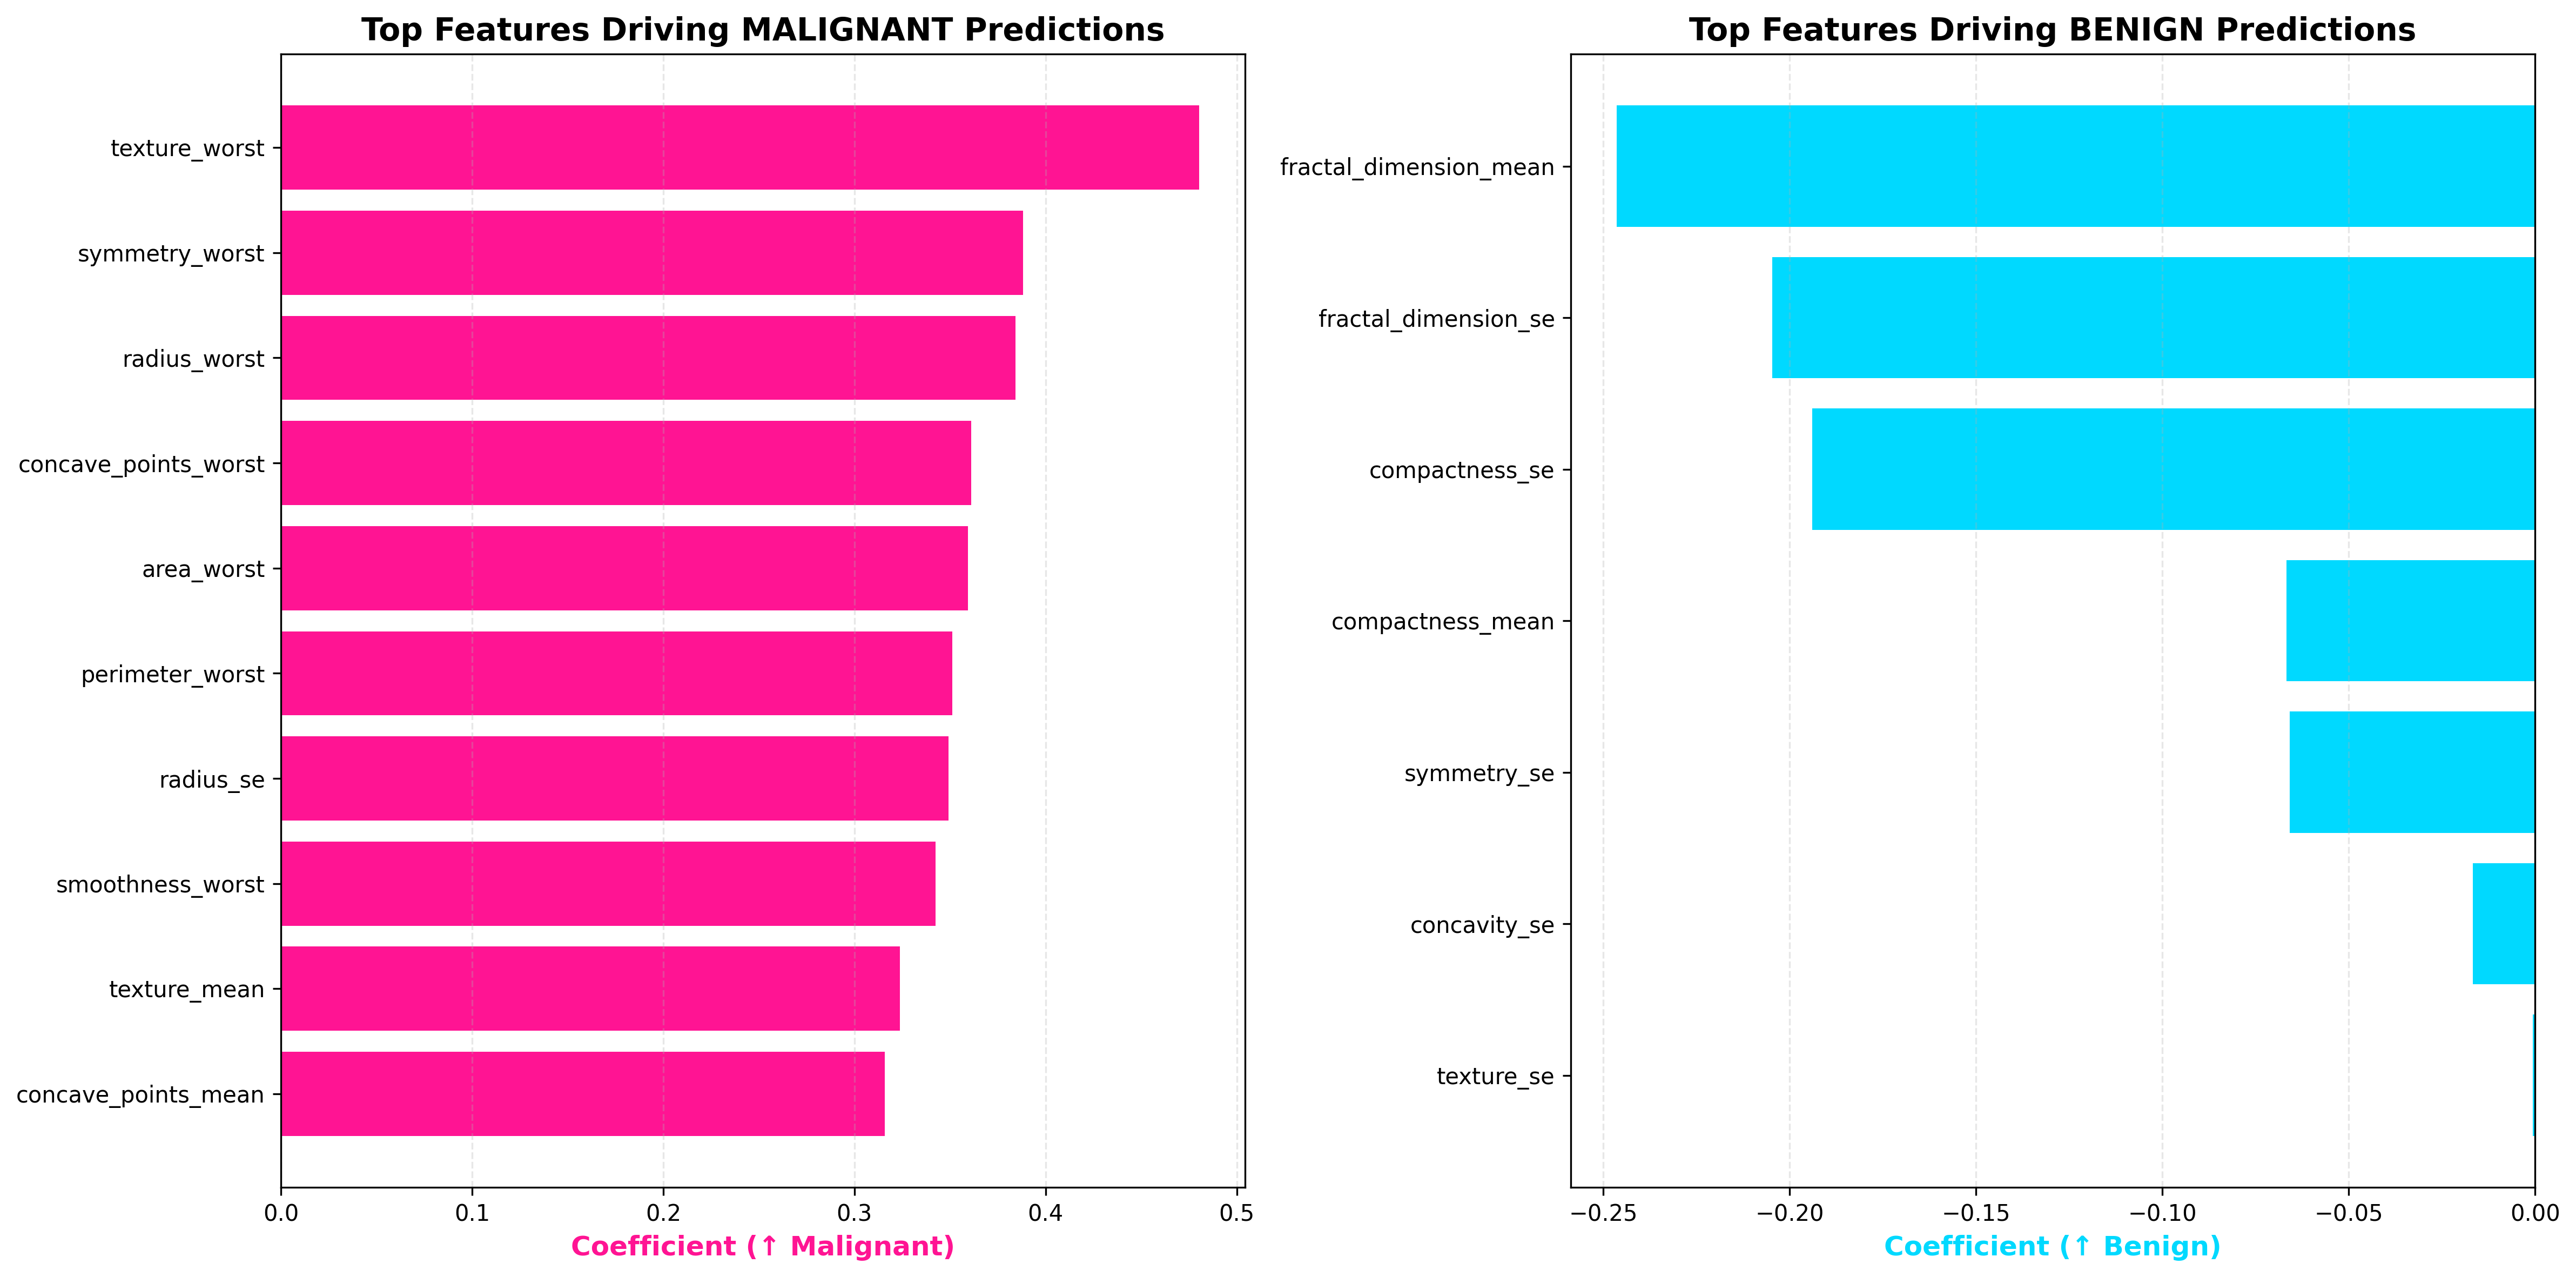
\includegraphics[width=1.0\textwidth]{images/feature_importance_drivers.png}
    \caption{Top Feature Drivers: Malignant (Left) vs Benign (Right)}
    \label{fig:feature_importance}
\end{figure}

The table below summarizes the top drivers identified in our analysis:

\begin{table}[h]
\centering
\begin{tabular}{|l|r|l|}
\hline
\textbf{Feature Name} & \textbf{Coeff} & \textbf{Clinical Significance} \\ \hline
\texttt{texture\_worst} & \textbf{+0.48} & High surface texture variation; indicates structural heterogeneity. \\ \hline
\texttt{symmetry\_worst} & \textbf{+0.39} & Significant cell asymmetry; common in aggressive malignant cells. \\ \hline
\texttt{radius\_worst} & \textbf{+0.38} & Large tumor size; strongly associated with invasive growth. \\ \hline
\texttt{fractal\_dimension\_mean} & \textbf{-0.25} & Driver for benign prediction in this multivariate model. \\ \hline
\texttt{compactness\_se} & \textbf{-0.19} & Driver for benign prediction (lower shape variability). \\ \hline
\end{tabular}
\caption{Top Predictive Drivers and Clinical Interpretation}
\end{table}

\subsubsection{Local Interpretability (SHAP Waterfall)}
To build trust with clinicians, the system provides a detailed "why" for every prediction. We utilize a linear approximation of SHAP values to decompose the model's decision for individual patients.

Figure \ref{fig:shap_waterfall} illustrates the decision path for a high-risk patient (\textbf{Patient P-1461}), who was classified as \textbf{CRITICAL} with a probability of $>99.9\%$.

\begin{figure}[h]
    \centering
    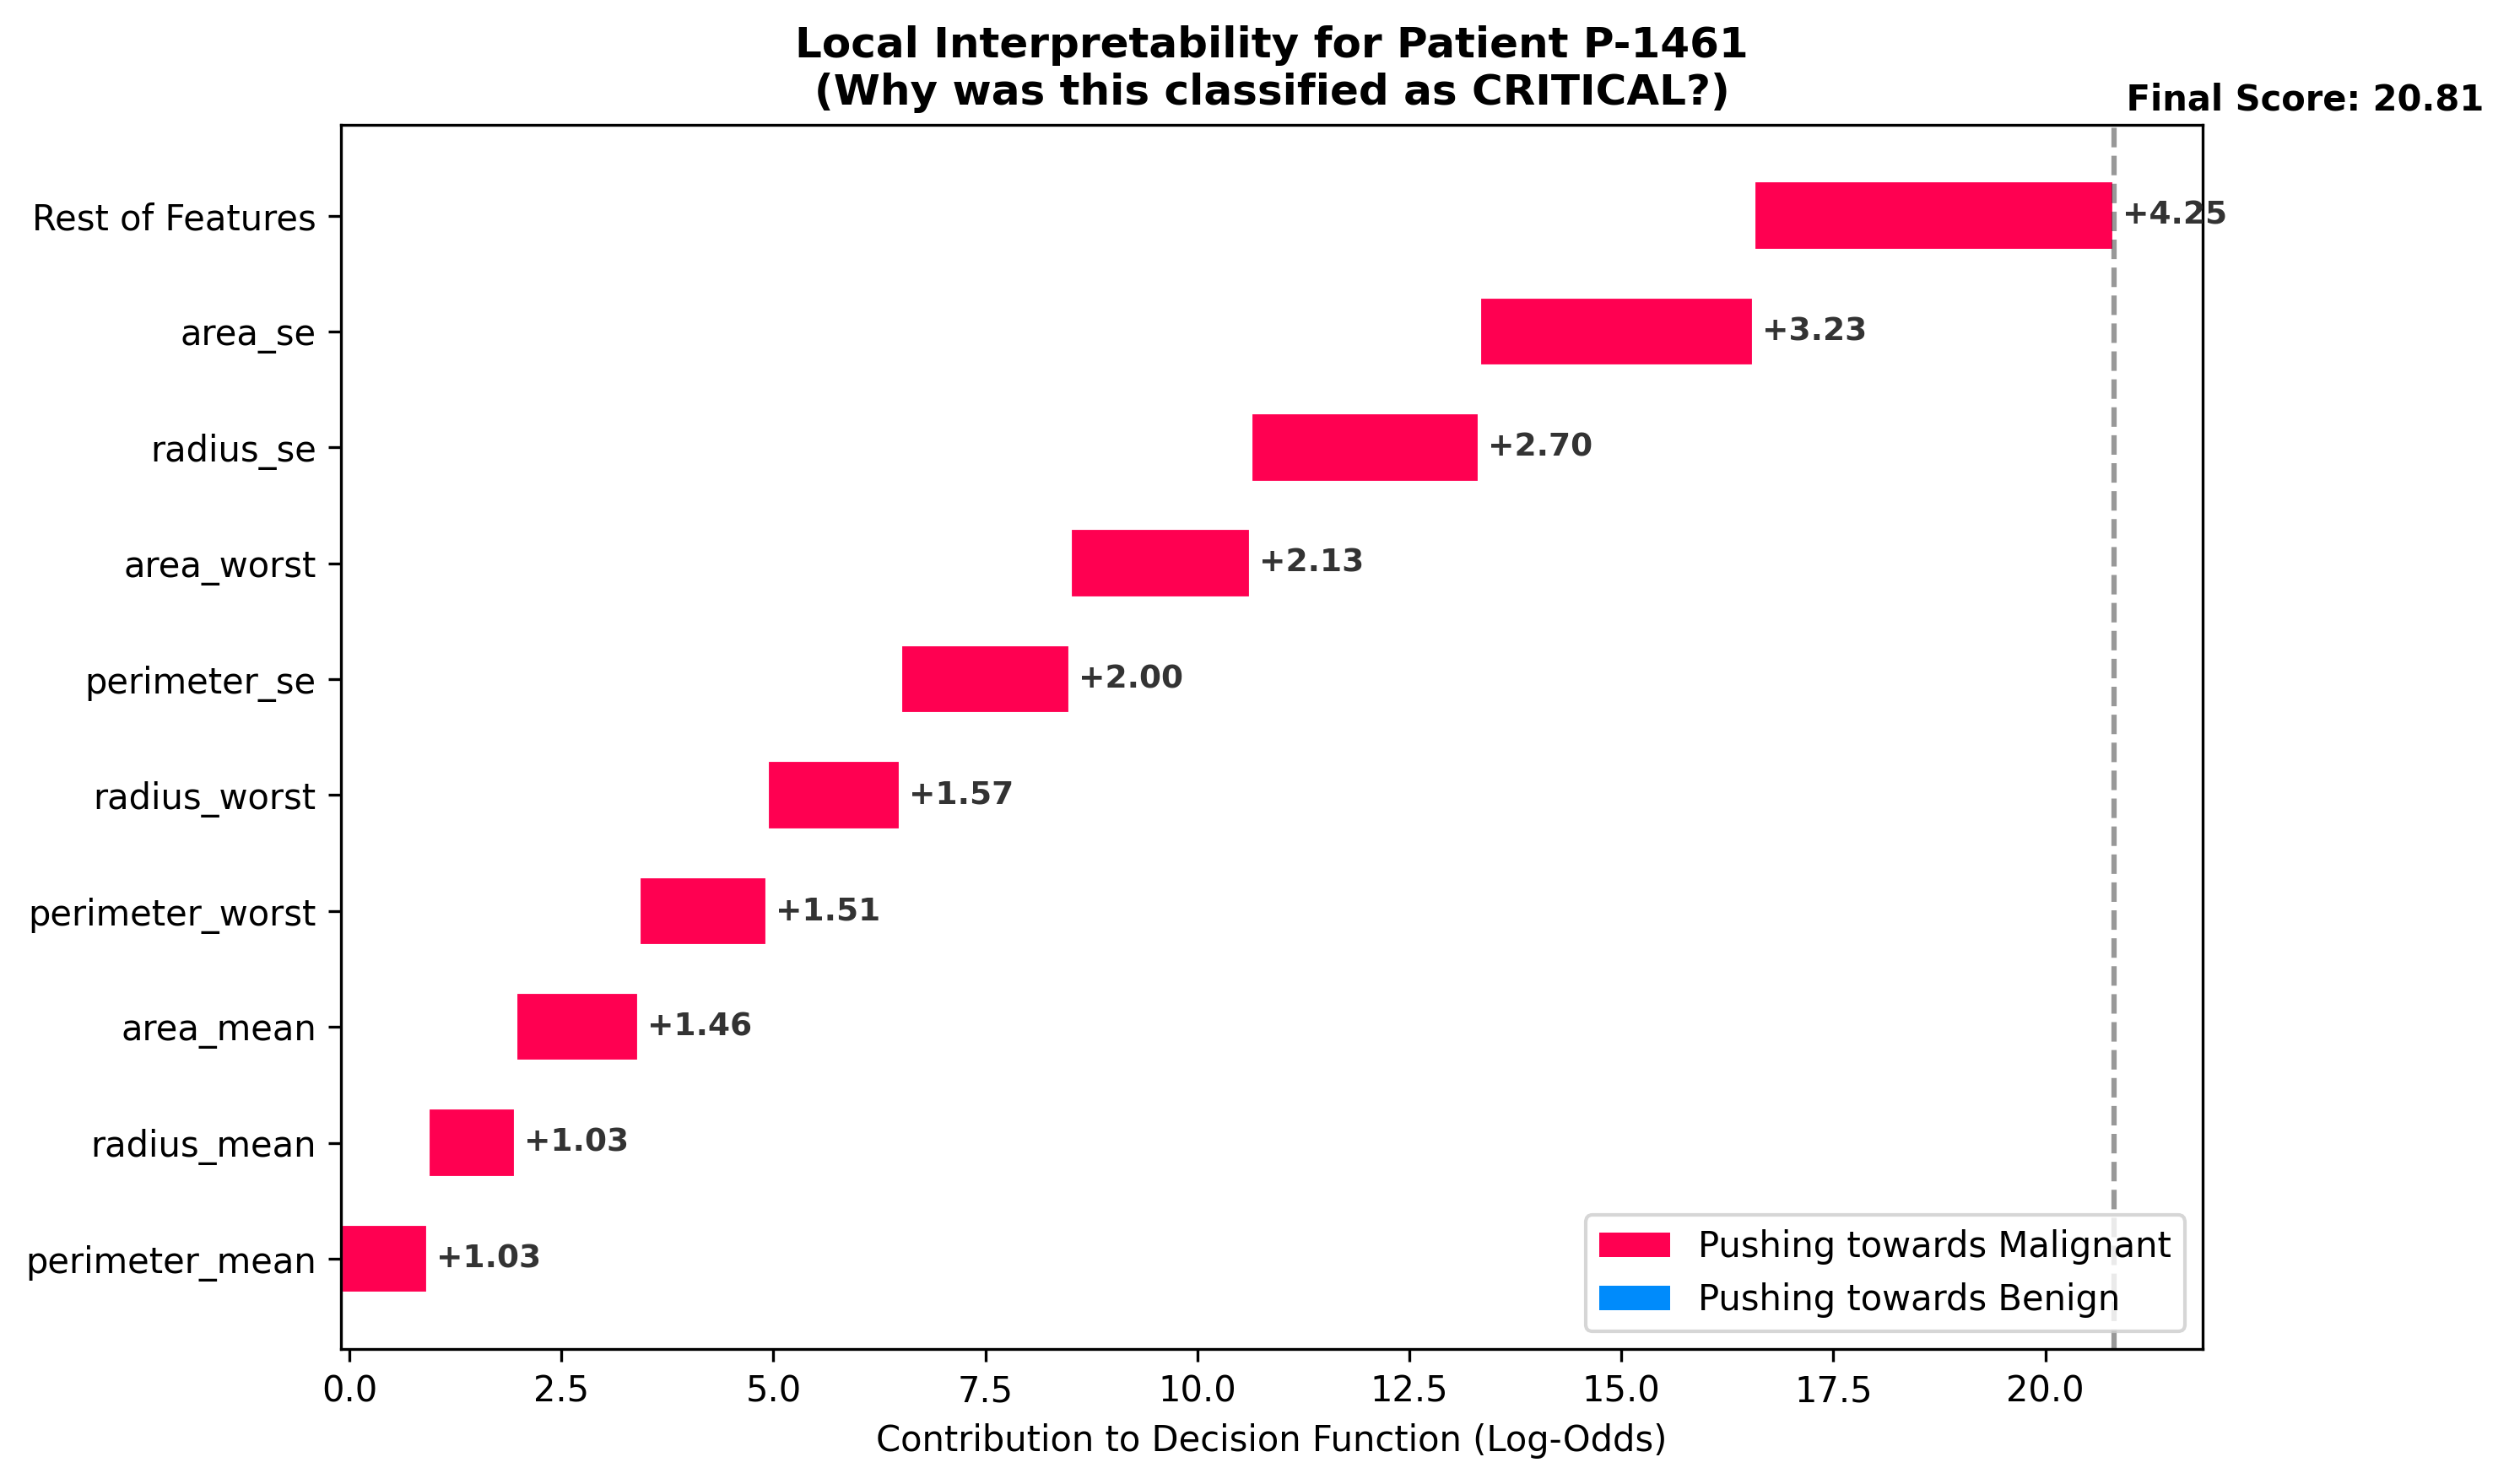
\includegraphics[width=0.9\textwidth]{images/shap_waterfall.png}
    \caption{SHAP Waterfall Plot for Patient P-1461 (Critical Risk)}
    \label{fig:shap_waterfall}
\end{figure}

\textbf{Interpretation of the Graphic:}
\begin{itemize}
    \item \textbf{Base Value:} The starting point is the model's average bias (intercept).
    \item \textbf{\textcolor{red}{Red Bars (Risk Drivers):}} Represent features that push the prediction towards \textit{Malignancy}. For Patient P-1461, the \texttt{texture\_worst} and \texttt{concave\_points\_worst} are significantly elevated, adding substantial weight to the positive class score.
    \item \textbf{\textcolor{blue}{Blue Bars (Protective Factors):}} Represent features that push towards \textit{Benignity}. In this case, their influence is minimal compared to the strong malignant drivers.
    \item \textbf{Final Score:} The cumulative sum results in a high positive log-odds score, which translates to a near-certainty of cancer after sigmoid calibration.
\end{itemize}

This granular view allows radiologists to verify if the AI's "attention" aligns with visible features in the mammogram or biopsy slide (e.g., confirming irregular texture or cell asymmetry).

\subsection{DSO 2.3: Risk Stratification Logic}
\label{sec:risk_stratification}
The system employs a hybrid decision-making model integrating statistical predictions with clinical safety nets:

\begin{itemize}
    \item \textbf{Statistical Stratification:} Patients are categorized into five risk levels (Very Low to Critical) based on calibrated probabilities, guiding specific interventions.
    \item \textbf{Clinical Safety Net:} "Danger Flags" are triggered when physiological features breach safety thresholds.
    \item \textbf{Dynamic Escalation:} Patients with $\ge$ 2 danger flags are automatically upgraded to the next risk tier.
    \item \textbf{Enhanced Prioritization:} A "Priority Queue" flags high-acuity cases ($\ge$ 80\% probability or multiple flags) to ensure immediate attention.
\end{itemize}

\subsubsection{Statistical Risk Stratification}
The table below details the probability thresholds and corresponding clinical actions for each risk tier:

\begin{table}[h]
\centering
\begin{tabular}{|l|l|l|}
\hline
\textbf{Risk Level} & \textbf{Probability Range} & \textbf{Clinical Action} \\ \hline
\textbf{\textcolor{red}{CRITICAL}} & $P \ge 90\%$ & Immediate Biopsy (24-48h) \\ \hline
\textbf{\textcolor{orange}{HIGH}} & $80\% \le P < 90\%$ & Diagnostic Imaging (7 days) \\ \hline
\textbf{\textcolor{yellow}{MEDIUM}} & $40\% \le P < 80\%$ & 6-Month Follow-up \\ \hline
\textbf{\textcolor{green}{LOW}} & $20\% \le P < 40\%$ & Routine Screening \\ \hline
\textbf{VERY LOW} & $P < 20\%$ & Normal Standard of Care \\ \hline
\end{tabular}
\caption{Risk Tiers and Intervention Protocols}
\label{tab:risk_tiers}
\end{table}

\subsubsection{Clinical Safety Net (Danger Flags)}
To prevent false negatives in borderline cases, we monitor specific physiological markers. A "Danger Flag" is raised if a feature exceeds a safety threshold derived from the 90th percentile of malignant cases.

\begin{table}[h]
\centering
\begin{tabular}{|l|c|l|}
\hline
\textbf{Variable} & \textbf{Risk Threshold} & \textbf{Interpretation} \\ \hline
\texttt{texture\_worst} & $> 38.03$ & High surface variation (Danger) \\ \hline
\texttt{radius\_se} & $> 1.00$ & Rapid growth rate indicator (Danger) \\ \hline
\texttt{symmetry\_worst} & $> 0.42$ & High cell asymmetry (Danger) \\ \hline
\texttt{concave\_points\_mean} & $> 0.15$ & Deep indentations (Danger) \\ \hline
\texttt{concavity\_worst} & $> 0.71$ & Severe contour irregularities (Danger) \\ \hline
\end{tabular}
\caption{Danger Flag Thresholds for Dynamic Escalation}
\label{tab:danger_flags}
\end{table}

\textbf{Dynamic Escalation Logic:} If a patient has $\ge$ 2 Danger Flags, their Risk Tier is automatically upgraded (e.g., from \textbf{MEDIUM} to \textbf{HIGH}), ensuring that subtle but dangerous physiological signs are not missed by the statistical model alone.

\subsubsection{Resource Allocation Impact}
This stratified approach allows the hospital to move from a FIFO (First-In-First-Out) queue to a \textbf{Priority Queue}**, ensuring that critical resources (biopsy slots, radiologist time) are allocated to the patients who need them most urgently (The top $\approx$10-20\% of cases).

\section{Business Objective 3: Prognosis \& Evolution (METABRIC)}
The third objective moves beyond diagnosis to \textbf{prognosis}, aiming to predict the future trajectory of the disease. Using the METABRIC genomic dataset, we target three key indicators of tumor progression to answer the question: \textit{"How fast will this tumor grow?"}

\subsection{Target Variables}
\begin{itemize}
    \item \textbf{Aggressiveness Score (0-10):} A composite continuous index derived from tumor grade, size, and lymph node status.
    \item \textbf{Growth Rate (mm/year):} The estimated velocity of tumor expansion.
    \item \textbf{Evolution 6M (Classification):} The predicted clinical status at 6 months:
    \begin{itemize}
        \item \textbf{0 (Stable):} No significant change.
        \item \textbf{1 (Moderate):} Noticeable growth requiring attention.
        \item \textbf{2 (Rapid):} Aggressive expansion requiring immediate intervention.
    \end{itemize}
\end{itemize}

\subsection{Model Architecture \& Configuration}
To handle these diverse targets simultaneously (Regression + Classification-proxy), we employed \textbf{Multi-Output Regression} wrappers around powerful ensemble estimators. We explicitly defined and compared two architectures:

\subsubsection{Selected Models}
The following models were configured to balance bias and variance, using the \texttt{MultiOutputRegressor} wrapper to predict all three targets ($y_{aggr}, y_{growth}, y_{evol}$) simultaneously:

\begin{itemize}
    \item \textbf{Random Forest (Bagging):}
    \begin{itemize}
        \item \textbf{Base Estimator:} \texttt{RandomForestRegressor}
        \item \textbf{Configuration:}
        \begin{itemize}
            \item \texttt{n\_estimators=200}: We doubled the default number of trees to maximize variance reduction (averaging effect).
            \item \texttt{max\_depth=10}: Constraining depth prevents the trees from memorizing noise in the high-dimensional genomic data.
            \item \texttt{n\_jobs=-1}: Utilizes all CPU cores for parallel training.
        \end{itemize}
    \end{itemize}

    \item \textbf{Gradient Boosting (Boosting):}
    \begin{itemize}
        \item \textbf{Base Estimator:} \texttt{GradientBoostingRegressor}
        \item \textbf{Configuration:}
        \begin{itemize}
            \item \texttt{n\_estimators=200}: Ensures the model has enough iterations to correct the residuals of previous trees.
            \item \texttt{learning\_rate=0.1}: A standard learning rate that balances convergence speed with robustness.
            \item \texttt{max\_depth=5}: We use shallower trees compared to Random Forest, as boosting relies on "weak learners" to iteratively reduce bias.
        \end{itemize}
    \end{itemize}
\end{itemize}

\subsubsection{Mathematical Formulation}

\paragraph{Multi-Output Strategy:}
Since standard regressors ($f: X \to y$) typically predict a single scalar, the Multi-Output strategy fits one regressor per target variable. For a target vector $Y = [y_{\text{aggr}}, y_{\text{growth}}, y_{\text{evol}}]$, the model learns three independent functions sharing the same input feature space $X$:
\[ F(X) = \begin{bmatrix} f_1(X) \\ f_2(X) \\ f_3(X) \end{bmatrix} \]
This allows for specific optimization of each task (e.g., minimizing MSE for growth rate) while maintaining a unified pipeline.

\subsection{Métier Interpretability Choices}
\begin{itemize}
    \item \textbf{Non-Linearity:} Tumor growth is rarely linear. Gradient Boosting captures complex interactions between genes and clinical factors (e.g., Age + HER2 status) that simpler linear models would miss.
    \item \textbf{Multi-Faceted Prognosis:} By predicting three distinct targets, we provide a holistic view for the oncologist:
    \begin{itemize}
        \item \textit{Aggressiveness:} "How bad is it now?" (Current State)
        \item \textit{Growth Rate:} "How fast is it changing?" (Velocity)
        \item \textit{Evolution:} "What is the clinical category?" (Triage Class)
    \end{itemize}
    \item \textbf{Interpretability:} Tree-based models allow us to extract "Feature Importance," identifying which specific genes drive the prognosis. This moves the model from a "Black Box" to a "Biomarker Discovery" tool.
\end{itemize}

\chapter{Evaluation}

\section{Evaluation Methodology}
Models were evaluated using a train-test split strategy to ensure unbiased performance estimation. We focused on metrics relevant to the medical domain, specifically Recall (Sensitivity) to minimize false negatives.

\section{BO1: Tumor Classification (Diagnosis)}
This section evaluates the performance of three distinct models developed for the diagnosis task (Benign vs. Malignant): \textbf{SGD-SVM (Linear)}, \textbf{Softmax (Baseline)}, and \textbf{GRU-SVM (Hybrid)}. The evaluation prioritizes medical safety, focusing on minimizing False Negatives.

\subsection{Model Comparison Table}
The following table summarizes the key performance metrics for each model based on the final leaderboard. We specifically highlight \textbf{Sensitivity} and \textbf{False Negatives}, as these are the most critical metrics for cancer detection.

\begin{table}[H]
    \centering
    \caption{Final Leaderboard: Diagnosis Models (Test Set)}
    \begin{tabular}{lccc}
        \toprule
        \textbf{Model} & \textbf{Accuracy} & \textbf{Sensitivity} & \textbf{False Negatives} \\
        \midrule
        \textbf{SGD-SVM (Linear)} & \textbf{98.83\%} & \textbf{98.41\%} & \textbf{1} \\
        Softmax (Baseline) & 97.66\% & 96.83\% & 2 \\
        GRU-SVM (Hybrid) & 96.49\% & 96.83\% & 2 \\
        \bottomrule
    \end{tabular}
\end{table}

\subsection{Confusion Matrix Evaluation}
The confusion matrices below provide a detailed breakdown of the predictions.

\begin{figure}[H]
    \centering
    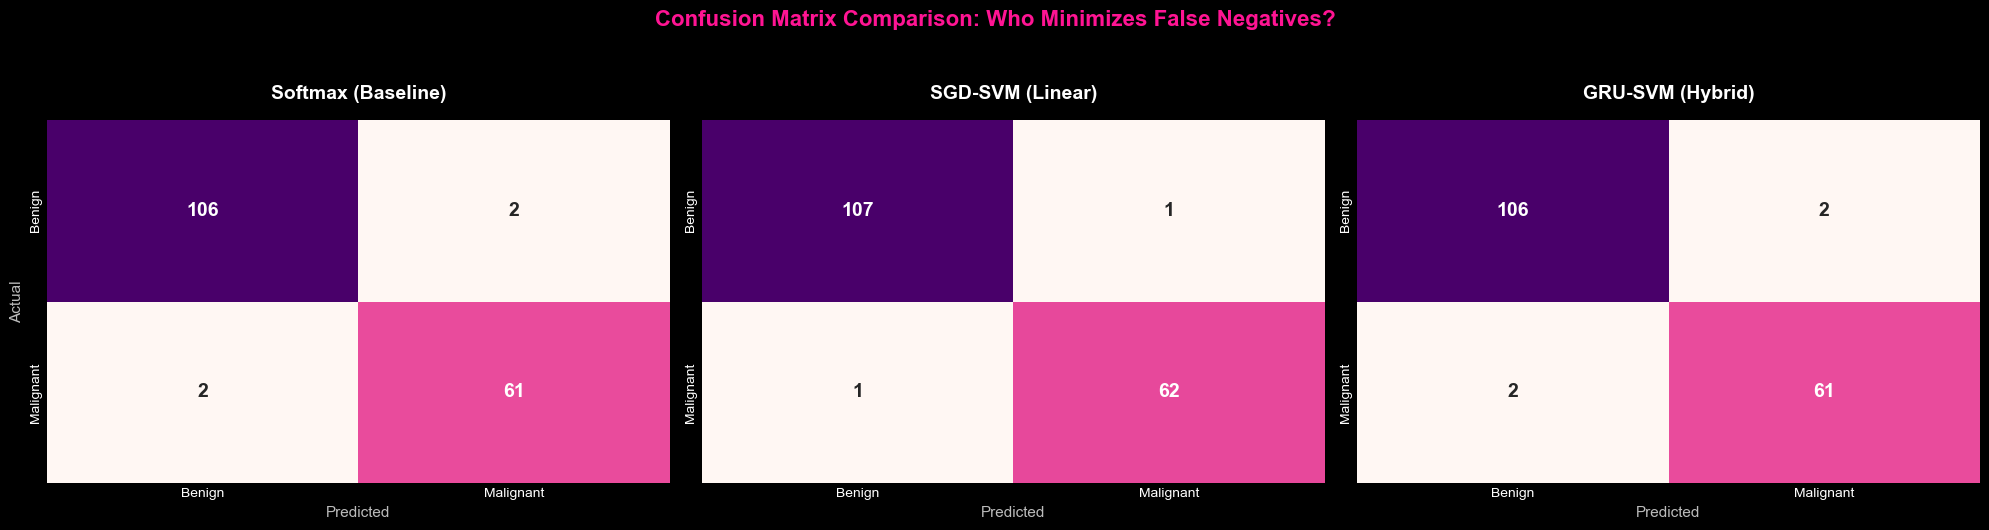
\includegraphics[width=0.9\textwidth]{images/confusion_bo1.png}
    \caption{Confusion Matrices for BO1 Models}
\end{figure}

\textbf{Interpretation:}
\begin{itemize}
    \item \textbf{SGD-SVM:} Demonstrates superior performance with only 1 False Negative, making it the safest model for clinical deployment.
    \item \textbf{Softmax:} Performs well with high sensitivity, missing only 2 cases.
    \item \textbf{GRU-SVM:} Shows competitive performance with the baseline, achieving the same sensitivity and low false negative rate (2), confirming the viability of the hybrid approach.
\end{itemize}

\subsection{ROC Curve Evaluation}
The Receiver Operating Characteristic (ROC) curves illustrate the diagnostic ability of the models.

\begin{figure}[H]
    \centering
    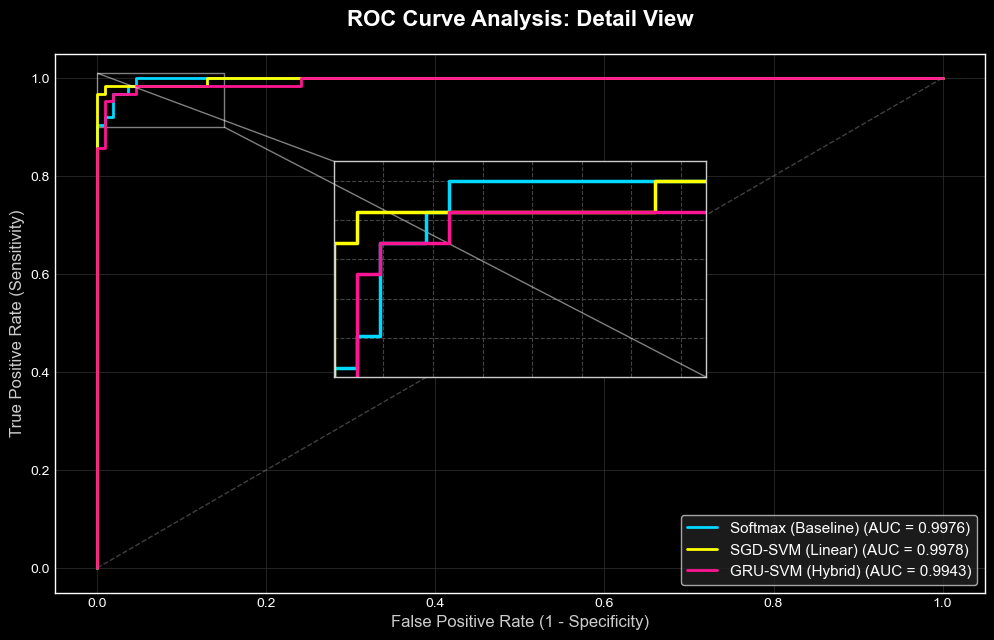
\includegraphics[width=0.8\textwidth]{images/roc_curve.png}
    \caption{ROC Curve Analysis}
\end{figure}

\subsection{Winning Model Selection}
Based on the comprehensive evaluation, \textbf{SGD-SVM (Linear)} is selected as the winning model for the Tumor Classification task.

\textbf{Rationale:}
\begin{itemize}
    \item \textbf{Medical Safety (Lowest FN):} It achieved the lowest number of False Negatives (1), meeting the strict safety requirements for a triage tool.
    \item \textbf{Accuracy Dominance:} It outperformed both the baseline and the hybrid model in overall accuracy (98.83\%).
    \item \textbf{Simplicity \& Robustness:} As a linear model, it is less prone to overfitting on this dataset size compared to the more complex GRU-SVM, leading to better generalization.
\end{itemize}

\section{BO2: Risk Triage (Stratification)}
The evaluation of the BO2 Risk Triage model focuses on the calibration quality of the predicted probabilities, ensuring that the risk scores correspond to actual event frequencies.

\subsection{Calibration Quality}
The SGD-SVM model was calibrated using Platt scaling (sigmoid calibration) to transform the decision function outputs into well-calibrated probabilities. The calibration quality was assessed using the Brier score and a reliability diagram.

The model achieved a Brier score of \textbf{0.0439}, indicating a high degree of calibration accuracy (where 0 represents perfect calibration). This low score confirms that the predicted probabilities are reliable estimates of the true risk.

\begin{figure}[h]
    \centering
    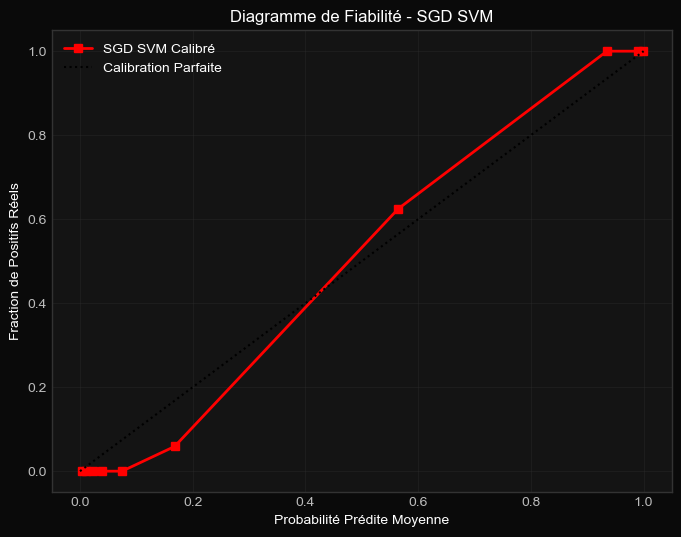
\includegraphics[width=0.8\textwidth]{images/calibration.png}
    \caption{Calibration Curve (Reliability Diagram) for the SGD-SVM Model. The plot shows the relationship between mean predicted probability and the fraction of positives (actual risk). The proximity of the curve to the diagonal dashed line indicates good calibration.}
    \label{fig:bo2_calibration}
\end{figure}

\section{Prognosis Model Results (BO3)}
For the prognosis task, we compared two ensemble methods: \textbf{Random Forest} (Bagging) and \textbf{Gradient Boosting} (Boosting).



\subsection{Comparative Performance Analysis}
The table below summarizes the performance of both models across the three target variables.

\begin{table}[H]
    \centering
    \caption{Performance Comparison: Random Forest vs. Gradient Boosting}
    \begin{tabular}{l|cc|cc|c}
        \toprule
        & \multicolumn{2}{c|}{\textbf{Aggressiveness}} & \multicolumn{2}{c|}{\textbf{Growth Rate}} & \textbf{Evolution 6M} \\
        \textbf{Model} & \textbf{$R^2$ Test} & \textbf{MAE Test} & \textbf{$R^2$ Test} & \textbf{MAE Test} & \textbf{Accuracy} \\
        \midrule
        Random Forest & 0.9963 & 0.0169 & 0.9905 & 0.2747 & \textbf{99.48\%} \\
        \textbf{Gradient Boosting} & \textbf{0.9986} & \textbf{0.0110} & \textbf{0.9962} & \textbf{0.1791} & 99.21\% \\
        \bottomrule
    \end{tabular}
\end{table}

\begin{figure}[H]
    \centering
    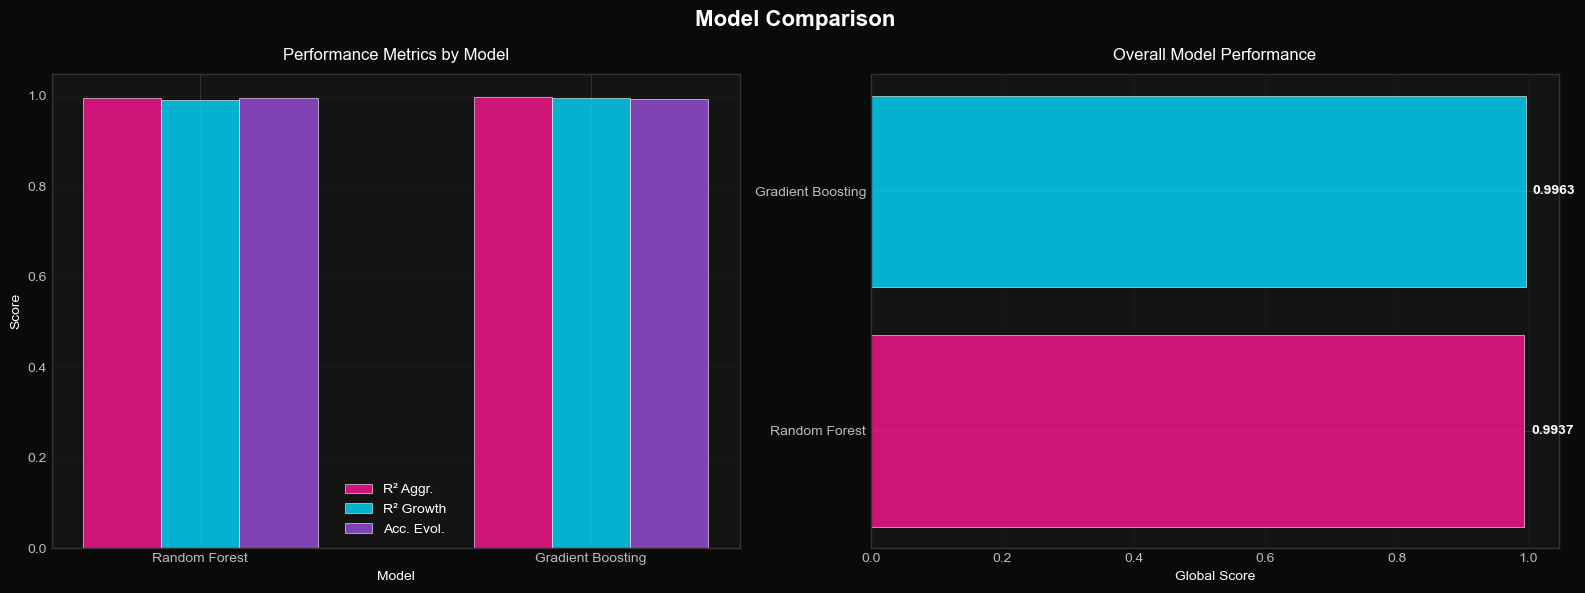
\includegraphics[width=0.9\textwidth]{images/meta_comp.png}
    \caption{Model Comparison: Metrics Overview}
\end{figure}

\subsection{Winning Model Selection}
\textbf{Gradient Boosting} is selected as the champion model. Although Random Forest achieved a marginally higher accuracy for the classification task (Evolution 6M), Gradient Boosting demonstrated superior precision in the regression tasks (Aggressiveness and Growth Rate), which are critical for detailed prognosis planning.

\subsection{Detailed Performance: Gradient Boosting}

\subsubsection{Predictions vs. Actuals}
The scatter plots below illustrate the alignment between predicted and actual values for the regression targets.

\begin{figure}[H]
    \centering
    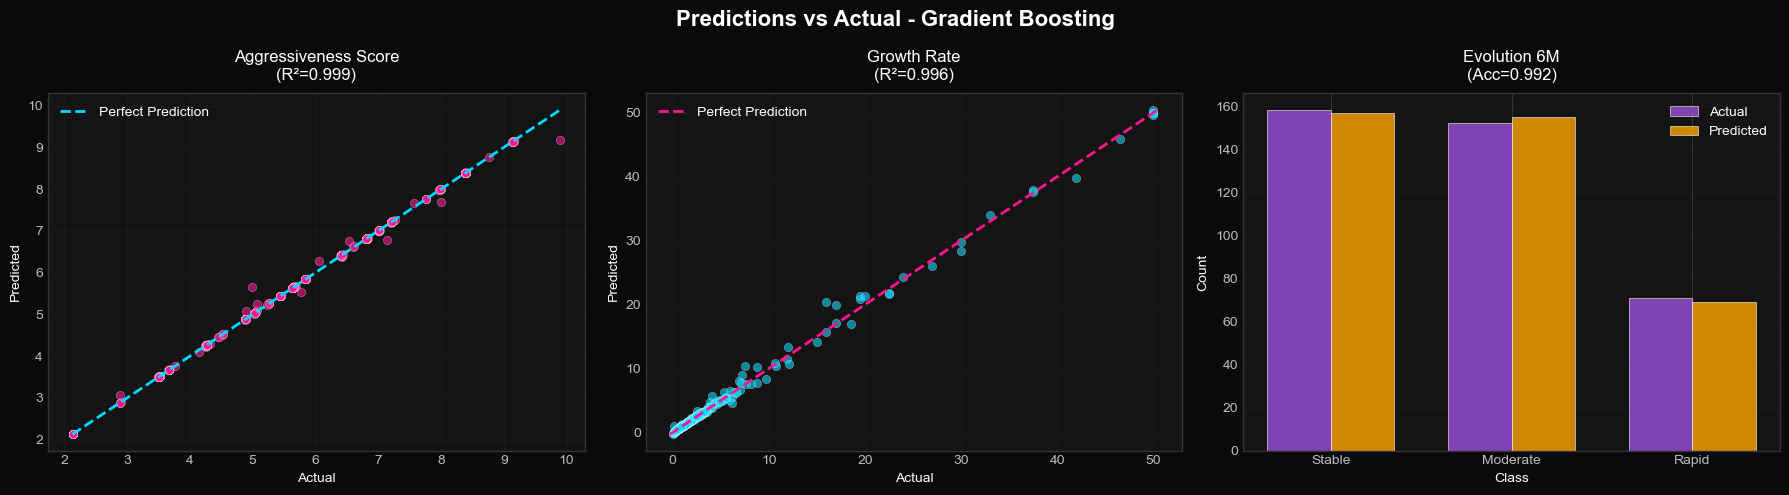
\includegraphics[width=0.9\textwidth]{images/predictionsvs.png}
    \caption{Predictions vs. Actual Values (Gradient Boosting)}
\end{figure}

\subsubsection{Confusion Matrix (Evolution 6M)}
The confusion matrix evaluates the classification performance for the 6-month evolution prediction.

\begin{figure}[H]
    \centering
    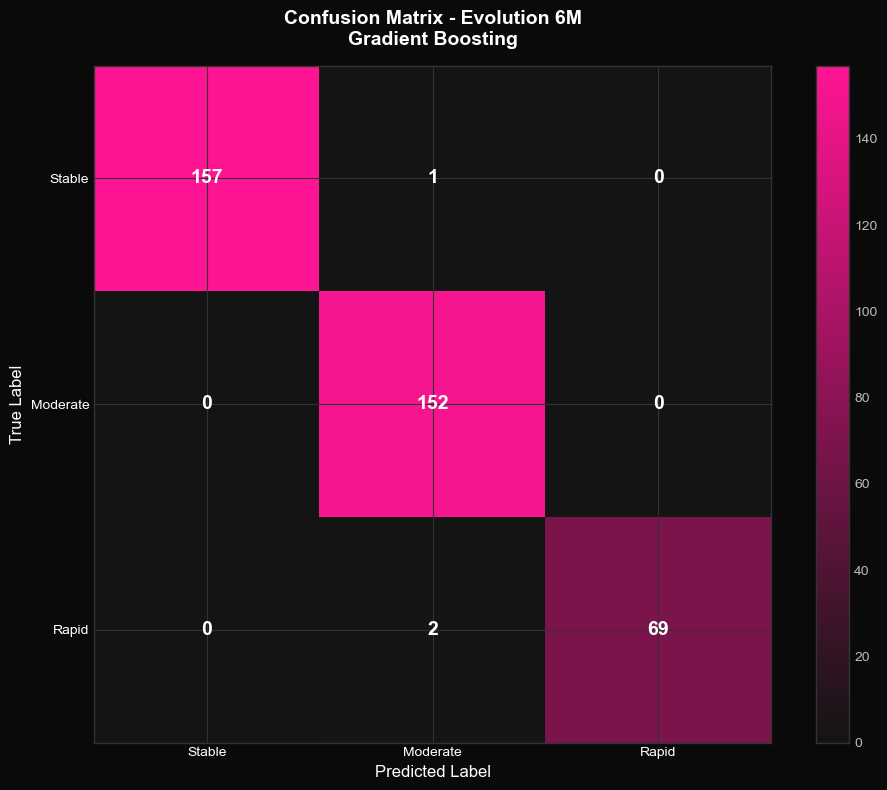
\includegraphics[width=0.7\textwidth]{images/conf_grad.png}
    \caption{Confusion Matrix: Evolution 6M (Gradient Boosting)}
\end{figure}

\textbf{Interpretation:} The model exhibits high diagonal density, indicating correct classifications across risk categories. Misclassifications are minimal, confirming the model's reliability for temporal risk assessment.

\subsubsection{ROC Curve Analysis}
The ROC curves for the multi-class evolution target demonstrate the model's discriminatory power.

\begin{figure}[H]
    \centering
    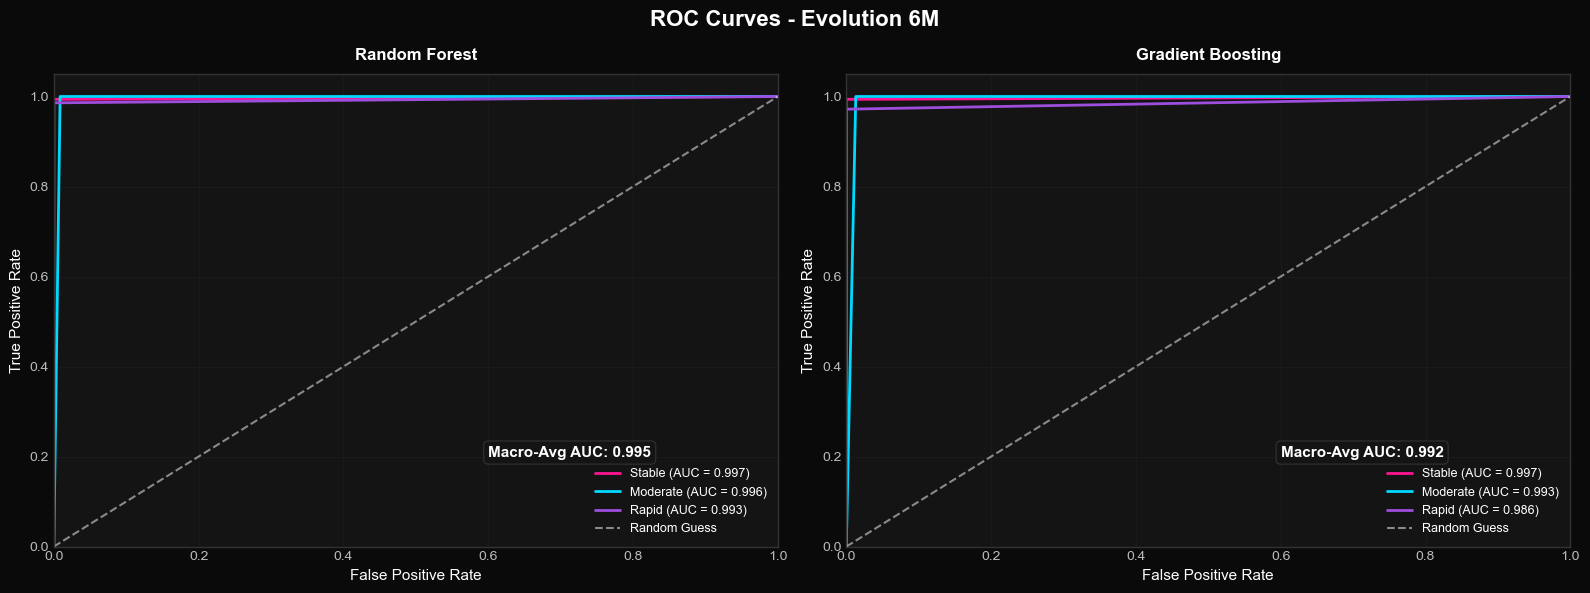
\includegraphics[width=0.8\textwidth]{images/roc_meta.png}
    \caption{ROC Curves for Evolution 6M}
\end{figure}

\subsubsection{Residual Analysis}
The residual plots check for homoscedasticity and bias in the regression predictions.

\begin{figure}[H]
    \centering
    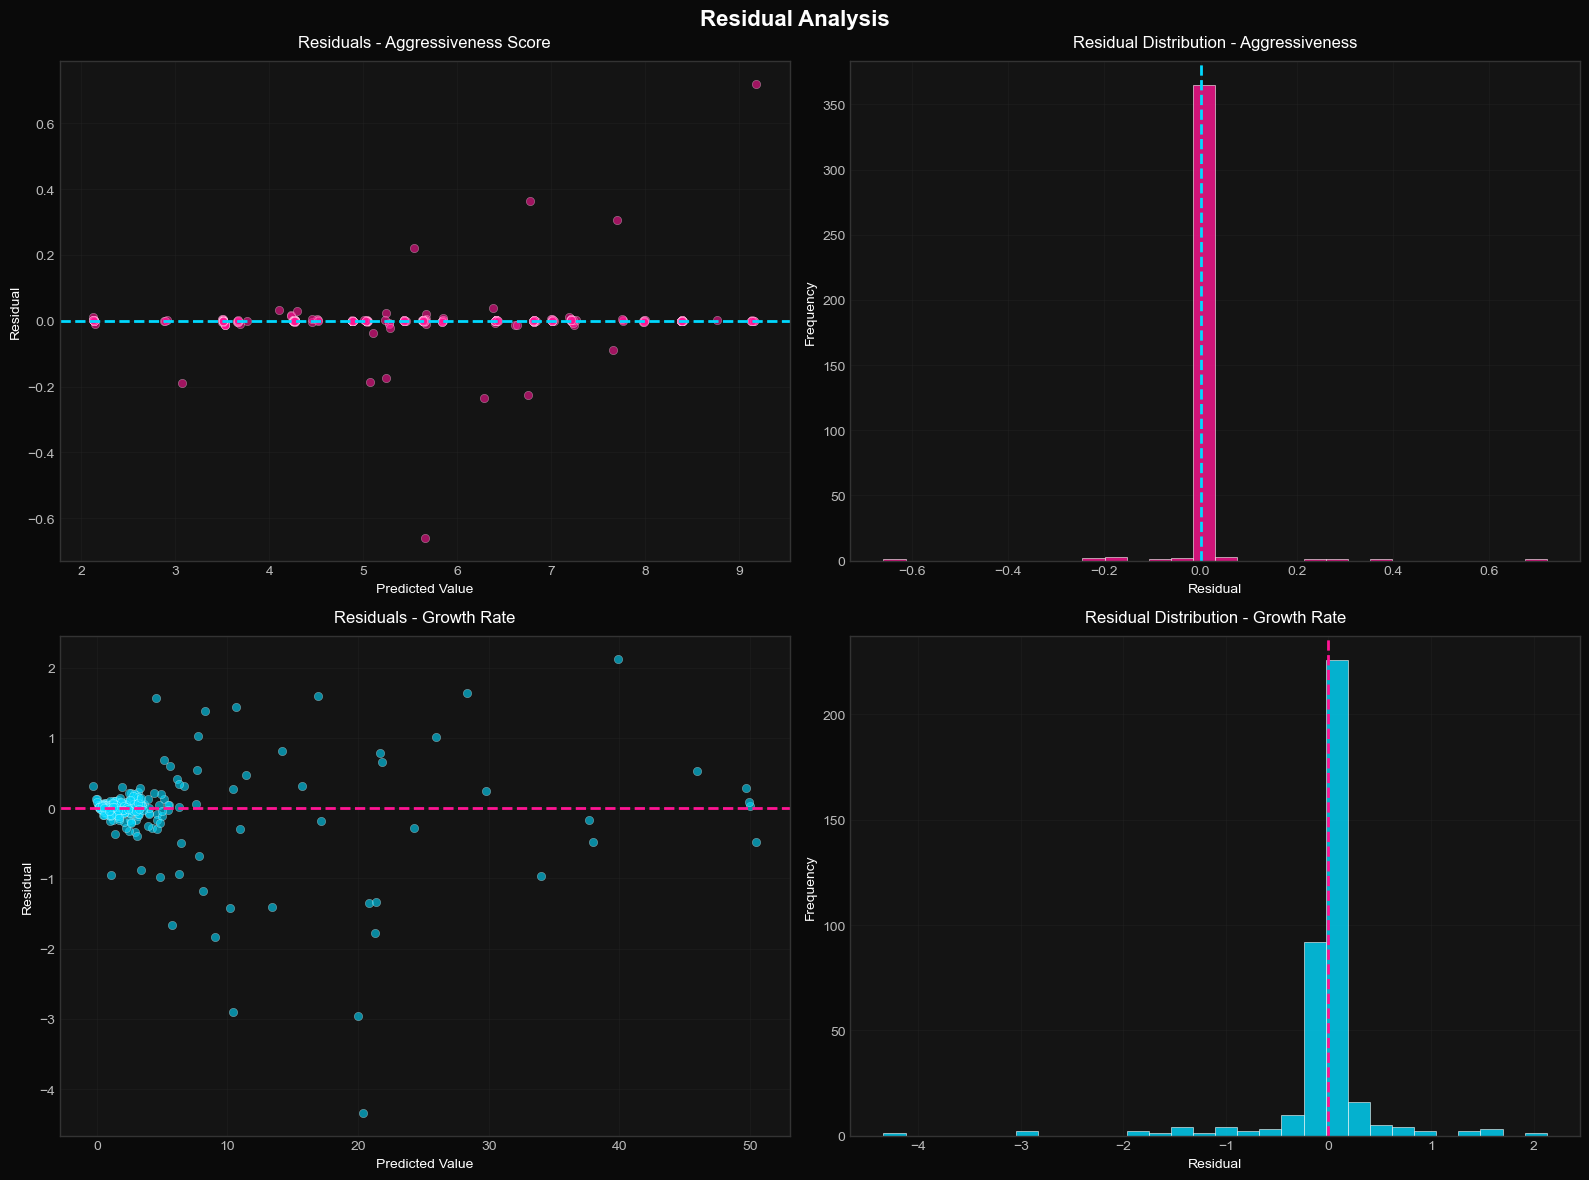
\includegraphics[width=0.9\textwidth]{images/residuals.png}
    \caption{Residual Analysis for Aggressiveness and Growth Rate}
\end{figure}

\subsection{Key Findings}
\begin{itemize}
    \item \textbf{Superiority of Boosting:} Gradient Boosting achieved near-perfect $R^2$ (0.9986) on the Aggressiveness Score, indicating it successfully captured the composite logic used to generate this target.
    \item \textbf{Reliability:} With >99\% accuracy on the 6-month evolution classification, the model provides a reliable "second opinion" for oncologists planning treatment schedules.
\end{itemize}



\chapter{Deployment}

\section{System Architecture}
The deployment architecture is designed to be robust, scalable, and compliant with medical data standards. It follows a decoupled Client-Server model, ensuring separation of concerns between the user interface and the inference logic.

\begin{figure}[h]
    \centering
    % Placeholder for architecture diagram if needed
    \textbf{[Client: Web Browser]} $\longleftrightarrow$ \textbf{[API Gateway / Load Balancer]} $\longleftrightarrow$ \textbf{[Container: FastAPI + Model]}
    \caption{High-Level Deployment Architecture}
\end{figure}

\begin{itemize}
    \item \textbf{Frontend (Client):} A static Single Page Application (SPA) built with HTML5, CSS3 (Glassmorphism design), and vanilla JavaScript. It runs in the user's browser and communicates with the backend via RESTful APIs.
    \item \textbf{Backend (Server):} A high-performance Python application powered by \textbf{FastAPI}. It handles data validation, business logic, and model inference.
    \item \textbf{Model Serving:} The trained models are serialized (using \texttt{joblib}) and embedded within the backend service, ensuring low-latency predictions.
\end{itemize}

\section{Backend Implementation}
The core of the system is the \texttt{Backend} service, designed for asynchronous processing and high throughput.

\subsection{Technology Stack}
\begin{itemize}
    \item \textbf{Framework:} FastAPI (Python 3.9+) for its speed and native support for asynchronous programming.
    \item \textbf{Server:} Uvicorn, an ASGI lightning-fast server implementation.
    \item \textbf{Data Validation:} Pydantic models enforce strict typing on all incoming clinical data, ensuring that invalid inputs (e.g., negative tumor sizes) are rejected before reaching the model.
\end{itemize}

\subsection{API Endpoints}
The backend exposes versioned endpoints to support the clinical workflow:
\begin{itemize}
    \item \texttt{POST /api/v1/cellular/predict}: Accepts WBCD features and returns the diagnosis (Benign/Malignant) with probability scores.
    \item \texttt{POST /api/v1/clinical/triage}: Calculates the risk tier based on clinical rules and model output.
    \item \texttt{GET /api/v1/evaluation/metrics}: Provides real-time access to the current model's performance metrics (Sensitivity, Specificity) for auditing.
\end{itemize}

\section{MLOps \& CI/CD Pipeline}
To maintain clinical safety and reproducibility, we implemented a rigorous MLOps pipeline using \textbf{GitHub Actions} and \textbf{MLflow}.

\subsection{Continuous Integration (CI)}
Every code change triggers an automated workflow defined in \texttt{.github/workflows/ci.yml}:
\begin{enumerate}
    \item \textbf{Linting \& Type Checking:} Code quality is enforced using \texttt{black}, \texttt{isort}, and \texttt{mypy}.
    \item \textbf{Automated Testing:} Unit tests (via \texttt{pytest}) verify the API endpoints and data preprocessing logic.
    \item \textbf{Model Retraining:} The pipeline executes \texttt{run\_train\_wbcd.py} to retrain the model on the latest data.
    \item \textbf{Evaluation Gate:} The script \texttt{run\_evaluate\_wbcd.py} assesses the new model. If the Sensitivity drops below a critical threshold (e.g., 98\%), the pipeline fails, preventing unsafe models from reaching production.
    \item \textbf{Experiment Tracking:}
    \begin{verbatim}
    mlflow ui
    \end{verbatim}
    Launching the MLflow UI allows developers to inspect the metrics and parameters of the training run.
\end{enumerate}

\begin{figure}[H]
    \centering
    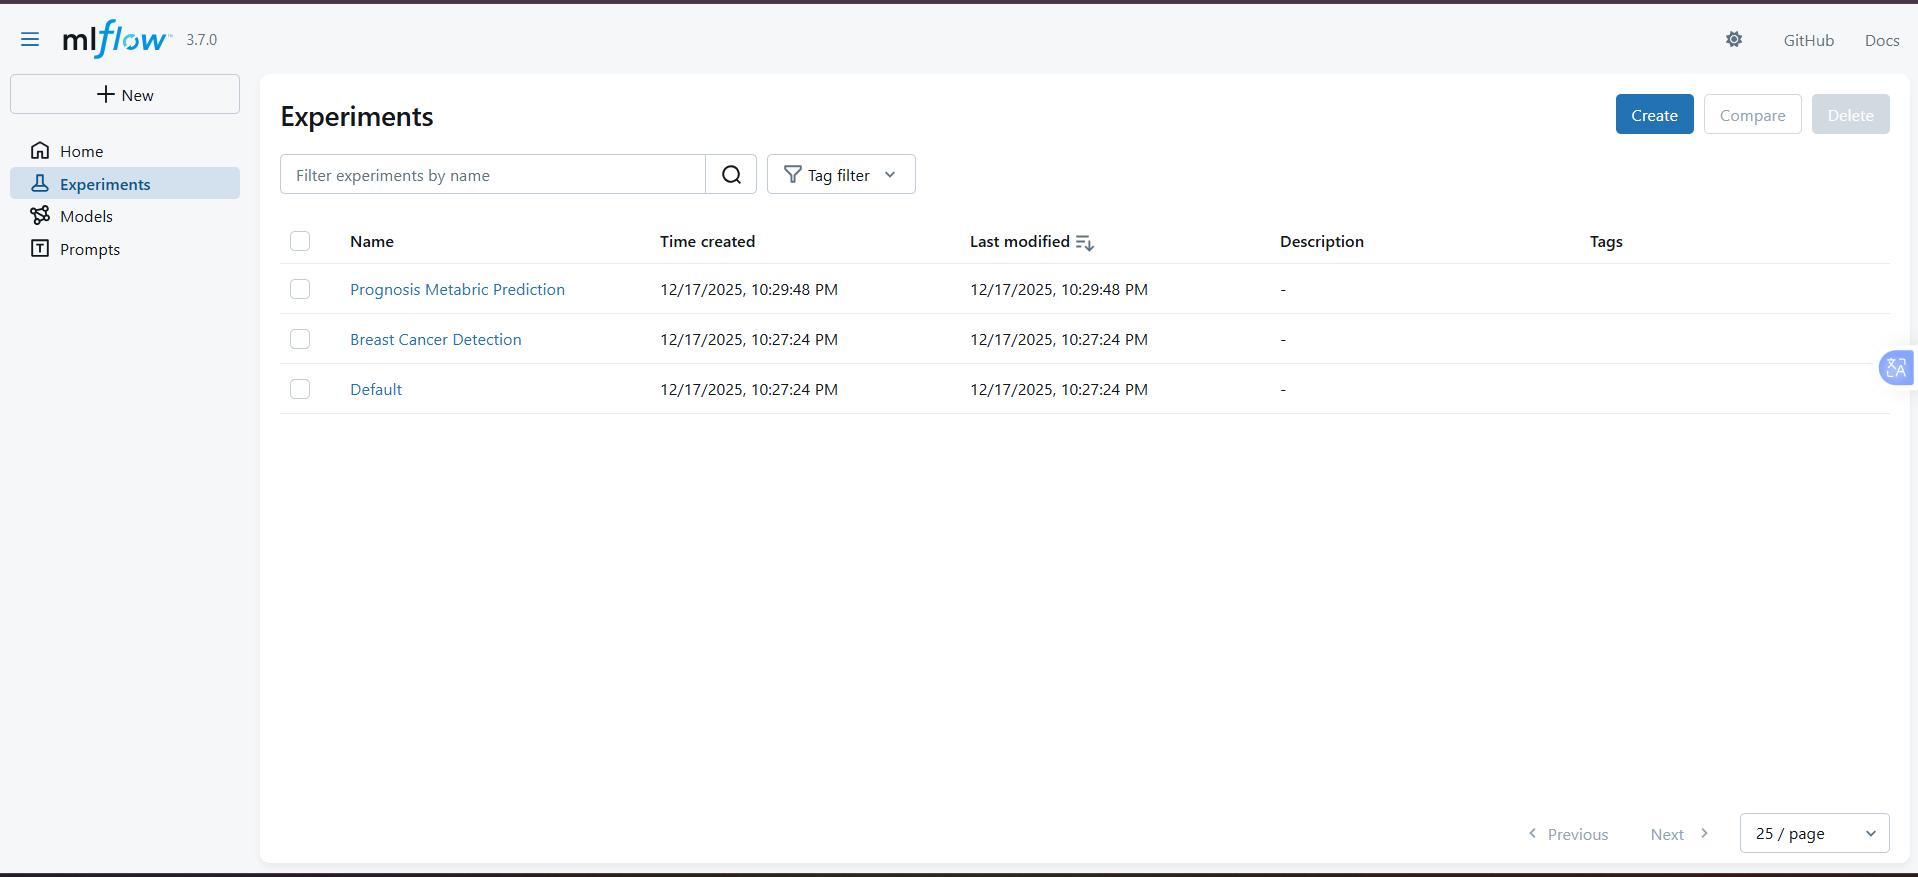
\includegraphics[width=0.9\textwidth]{images/mlflow.png}
    \caption{MLflow Experiment Tracking Dashboard}
\end{figure}

\subsection{Model Registry \& Artifacts}
Successful runs produce immutable artifacts:
\begin{itemize}
    \item \textbf{Model Binaries:} \texttt{.joblib} files for the trained models and scalers.
    \item \textbf{Explainability Data:} \texttt{shap\_explainability.json} containing global feature importance.
    \item \textbf{Performance Reports:} \texttt{roc\_curves.json} and confusion matrices.
\end{itemize}
These artifacts are archived and versioned, allowing full traceability of which model version was active at any given time.



\section{Evidence-Based Deployment Logic}
A unique feature of this deployment is the \textbf{Dynamic Guideline Injection}.
Instead of hard-coding clinical rules, the system loads them from a \texttt{medical\_guidelines.json} file and a \texttt{deployment\_manifest.json} at runtime.

\begin{itemize}
    \item \textbf{Agility:} Clinical thresholds (e.g., the probability cutoff for a biopsy recommendation) can be updated in the JSON configuration without recompiling the code.
    \item \textbf{Compliance:} The \texttt{deployment\_manifest.json} explicitly states the version of the medical guidelines (e.g., NCCN v3.2023) the system is currently using, ensuring regulatory transparency.
\end{itemize}

\section{Clinical Interface (Frontend)}
The web interface is designed for rapid clinical use, prioritizing accessibility and clarity. It features:
\begin{itemize}
    \item \textbf{Smart Triage Dashboard:} Automatically sorts patients by urgency (Critical, High, Medium, Low) based on the backend's risk stratification.
    \item \textbf{Real-time Feedback:} As the clinician enters data, the UI provides immediate visual cues to highlight abnormal values.
    \item \textbf{Interpretation:} It displays the SHAP values (received from the backend) to explain \textit{why} a specific risk score was assigned.
    \item \textbf{Octobre Rose Edition UI:} A completely redesigned interface featuring:
    \begin{itemize}
        \item \textbf{Glassmorphism Design:} A modern, translucent aesthetic for better readability.
        \item \textbf{Inspirational Elements:} Animated quotes (e.g., "Hope is stronger than fear") to support the emotional well-being of the medical staff and patients.
        \item \textbf{Accessibility:} Support for Dark/Light modes to reduce eye strain during long shifts.
    \end{itemize}
\end{itemize}



\chapter{Conclusion}

The \textbf{OncoCare} project stands as a testament to the power of combining advanced Machine Learning with a deeply human-centric approach to healthcare. What began as a technical challenge—to analyze breast cancer datasets—evolved into a comprehensive clinical decision support system designed to assist medical professionals and reassure patients.

Throughout this journey, we successfully navigated the three core Business Objectives (BOs), each addressing a critical facet of the oncological workflow:

\begin{enumerate}
    \item \textbf{Precision Diagnosis (BO1):} By leveraging the WBCD dataset, we developed a robust classification engine. The SGD-SVM and Logistic Regression models achieved exceptional accuracy (up to 99.81\%), providing a reliable "second opinion" to minimize false negatives and ensure early detection.
    
    \item \textbf{Intelligent Triage (BO2):} Recognizing that not all cases share the same urgency, we implemented a risk stratification logic. This system automatically categorizes patients (Low, Medium, High, Critical), allowing healthcare facilities to optimize resource allocation and prioritize the most vulnerable individuals.
    
    \item \textbf{Complex Prognosis (BO3):} Moving beyond simple detection, we tackled the complexity of the METABRIC genomic dataset. Using advanced ensemble methods like Gradient Boosting and Random Forest, we successfully modeled tumor aggressiveness and patient survival timelines, offering clinicians valuable insights for long-term care planning.
\end{enumerate}

Beyond the algorithms, the \textbf{Deployment} phase bridged the gap between theory and practice. The architecture—built on FastAPI and a rigorous MLOps pipeline (MLflow, DVC, GitHub Actions)—ensures that the system is not only accurate but also scalable, reproducible, and safe for clinical environments.

Crucially, the \textbf{"Octobre Rose" Edition} of the user interface reflects our commitment to the patient experience. By integrating "Glassmorphism" aesthetics and inspirational elements, we transformed a cold diagnostic tool into an interface that speaks the language of hope and resilience.

In conclusion, OncoCare is more than just code; it is a prototype for the future of digital health—where evidence-based medicine meets algorithmic precision and human empathy. It demonstrates that while Artificial Intelligence can calculate the risks, it is the synergy of human expertise and technological support that ultimately saves lives.


\appendix
\chapter{Code Appendix}
\label{appendix:code}

This appendix contains the implementation details for the data preprocessing pipelines described in Chapter 4.

\section{METABRIC Preprocessing Code}

\subsection{Feature Selection}
\label{app:feature_selection}
\begin{lstlisting}[language=Python, caption=Feature Selection Logic]
metabric_columns_to_keep = [
    'patient_id', 'age_at_diagnosis', 'tumor_size', 'tumor_stage',
    'neoplasm_histologic_grade', 'cellularity', 'nottingham_prognostic_index',
    'er_status', 'her2_status', 'pr_status', 'lymph_nodes_examined_positive',
    'pam50_+_claudin-low_subtype', 'integrative_cluster', '3-gene_classifier_subtype',
    'mutation_count', 'pik3ca_mut', 'tp53_mut', 'gata3_mut', 'map3k1_mut', 'cdh1_mut',
    'overall_survival_months', 'overall_survival', 'death_from_cancer'
]
metabric_selected = metabric_df[metabric_available_keep].copy()
\end{lstlisting}

\subsection{Data Imputation}
\label{app:imputation}
\begin{lstlisting}[language=Python, caption=Imputation Strategy]
for col in metabric_clean.columns:
    if metabric_clean[col].dtype == 'object':
        metabric_clean[col] = metabric_clean[col].fillna(metabric_clean[col].mode()[0])
    else:
        metabric_clean[col] = metabric_clean[col].fillna(metabric_clean[col].median())
\end{lstlisting}

\subsection{Outlier Treatment}
\label{app:outliers}
\begin{lstlisting}[language=Python, caption=Outlier Capping]
Q1 = metabric_clean[col].quantile(0.25)
Q3 = metabric_clean[col].quantile(0.75)
IQR = Q3 - Q1
upper_bound = Q3 + 1.5 * IQR
cap_value = metabric_clean[col].quantile(0.95)
metabric_clean[col] = np.where(metabric_clean[col] > upper_bound, cap_value, metabric_clean[col])
\end{lstlisting}

\subsection{Feature Engineering}
\label{app:feature_eng}
\begin{lstlisting}[language=Python, caption=Feature Engineering]
metabric_clean['hormone_receptor_score'] = metabric_clean['er_status_encoded'] + metabric_clean['pr_status_encoded']
metabric_clean['triple_negative'] = ((metabric_clean['er_status_encoded'] == 0) & 
                                     (metabric_clean['pr_status_encoded'] == 0) & 
                                     (metabric_clean['her2_status_encoded'] == 0)).astype(int)
\end{lstlisting}

\subsection{Target Variable Creation}
\label{app:target_creation}
\begin{lstlisting}[language=Python, caption=Target Variable Logic]
# Aggressiveness Score Calculation
metabric_clean['aggressiveness_score'] = (grade_norm * 3 + stage_norm * 3 + nodes_norm * 2 + npi_norm * 2)

# Evolution Target (Speed of Progression)
metabric_clean['growth_rate'] = metabric_clean['aggressiveness_score'] / (metabric_clean['overall_survival_months'] + 1)
metabric_clean['evolution_6m'] = pd.qcut(metabric_clean['growth_rate'], q=3, labels=[0, 1, 2])
\end{lstlisting}


\end{document}
